\documentclass{beamer}


% ==============================================================
% Theme Selection (METU colors: maroon/red & white via Ritsumeikan.sty)
% ==============================================================
\usetheme{Madrid}
\usecolortheme{beaver}
\usefonttheme{professionalfonts}

% Packages
\usepackage[utf8]{inputenc}
\usepackage[T1]{fontenc}
\usepackage{hyperref}
\usepackage{graphicx,bm}
\usepackage{latexsym,amssymb,amsfonts,amsmath,xcolor,multicol,booktabs,braket}
\usepackage{color}
\usepackage{caption}
\usepackage{subcaption}
\usepackage{array}
\usepackage{forest}
\usepackage{Ritsumeikan}
\usepackage{tikz}
\usetikzlibrary{tikzmark, arrows.meta, positioning, calc, decorations.pathreplacing}
\usepackage[square,sort,comma,numbers]{natbib}
\setbeamertemplate{navigation symbols}{}

% --------------------------------------------------------------
% A few METU-flavoured accent colours that harmonise with the
% maroon "ritsumeikan" colour defined in the style file.
% --------------------------------------------------------------
\definecolor{metured}{RGB}{128,0,0}
\definecolor{metuaccent}{RGB}{176,40,40}
\definecolor{metugold}{RGB}{196,142,40}
\definecolor{metugray}{RGB}{90,90,90}
\definecolor{metulight}{RGB}{245,238,238}

% Highlight box helper
\newcommand{\hl}[1]{{\color{metured}\textbf{#1}}}
\newcommand{\new}[1]{{\color{metuaccent}\textbf{#1}}}

% Ensure the title-page text reads clearly (white) on the maroon title box
\setbeamercolor{title}{bg=metured,fg=white}
\setbeamercolor{subtitle}{fg=white}
\setbeamercolor{author}{fg=black}
\setbeamercolor{institute}{fg=black}
\setbeamercolor{date}{fg=black}

% A small "NEW" flag to mark the fresh material on a slide title
\newcommand{\newflag}{\hfill{\footnotesize\colorbox{metugold}{\color{white}\bfseries\,NEW\,}}}

% Math shortcuts
\newcommand{\sixj}[6]{\left\{ \begin{matrix} #1 & #2 & #3 \\ #4 & #5 & #6 \end{matrix} \right\}}
\newcommand{\Tr}{\mathrm{Tr}\,}
\newcommand{\dbk}[1]{\langle\langle #1 \rangle\rangle}

% Title Information
\title[Quantum Chaotic Dynamics in Matrix Models]{Explanation of Quantum Chaotic Dynamics in Matrix Gauge Theories}
\subtitle{PhD Thesis Committee Report}
\author[Berk Özcan]{Berk Özcan \\ \small Supervisor: Prof. Dr. Seçkin Kürkçüoğlu}
\institute[METU]{Middle East Technical University \\ Department of Physics}
\date{May 2024 -- May 2027}

\begin{document}

% ==============================================================
% Slide 1: Title
% ==============================================================
{
\setbeamertemplate{footline}{}
\setbeamertemplate{headline}{}
\begin{frame}
  \titlepage
  \begin{center}
    \vspace{-0.8em}
    
\includegraphics[height=1.7cm]{pic/METU_logo.png}
  \end{center}
\end{frame}
}

% ==============================================================
% Slide 2: Outline
% ==============================================================
\begin{frame}{Outline}
  \tableofcontents
\end{frame}

% ==============================================================
% Section 1: Introduction & Motivation
% ==============================================================
\section{Introduction \& Motivation}

\begin{frame}{Motivation: Chaos, Gravity, and the MSS Bound}
  \begin{itemize}
    \item \hl{Gauge--gravity duality} links chaotic quantum systems to black-hole physics, motivating the study of chaos in matrix models.
    \item \textbf{Measuring chaos:}
    \begin{itemize}
      \item \emph{Classical:} Lyapunov exponents $\to$ exponential divergence of phase-space trajectories.
      \item \emph{Quantum:} Out-of-Time-Ordered Correlators (OTOCs), $C(t)=\braket{[\hat W(t),\hat V(0)]^2}\sim e^{2\lambda_L t}$.
    \end{itemize}
    \item \hl{The MSS bound} (Maldacena--Shenker--Stanford): a universal upper bound on quantum chaos
    \begin{equation*}
      \lambda_L \le \frac{2\pi k_B T}{\hbar}.
    \end{equation*}
    Black holes are expected to \emph{saturate} it; the SYK model does, and BFSS/BMN are conjectured to.
  \end{itemize}
\end{frame}

\begin{frame}{Thesis Goals}
  \begin{block}{Primary Goal}
    Study \textbf{real-time quantum dynamics} starting from (near-)thermal-equilibrium configurations in matrix models with fuzzy-sphere geometry ($S_F^2\times\mathbb{R}$) and in the string-theoretic \new{BMN model}.
  \end{block}
  \vspace{-0.8em} \begin{block}{Specific Objectives} \begin{enumerate}
      \item Apply the \hl{Gaussian State Approximation (GSA)} to the Heisenberg EOM $\Rightarrow$ truncated EOM for 1- and 2-point correlators.
      \item Determine the thermal equation of state by \hl{von Neumann entropy maximization}.
      \item Solve the truncated EOM numerically and extract the largest Lyapunov exponent $\lambda_L$.
      \item Probe the \new{MSS bound}, the \new{Bekenstein bound}, and \new{entanglement dynamics}.
    \end{enumerate}
  \end{block}
\end{frame}

\begin{frame}{What is New Since the Last Report}
  \begin{columns}[T]
    \begin{column}{0.5\textwidth}
      \begin{block}{Bosonic model -- now \emph{completed}}
        \begin{itemize}
          \item \new{Non-planar interaction term} included (full $O(2)$ model, not just planar $D_4$).
          \item \new{Entropy} \& Bekenstein-bound analysis.
          \item \new{Entanglement entropy} dynamics ($\lambda_E$ vs $\lambda_L$).
          \item Manuscript prepared for submission.
        \end{itemize}
      \end{block}
    \end{column}
    \begin{column}{0.5\textwidth}
      \begin{block}{BMN model -- \emph{ongoing}}
        \begin{itemize}
          \item Full GSA EOM derived (cubic Myers term!).
          \item Non-trivial fuzzy-sphere vacuum $\bar X_a\neq 0$.
          \item $SO(3)\times SO(6)$ thermal equilibrium \& gap equations.
        \end{itemize}
      \end{block}
    \end{column}
  \end{columns}
  \vspace{0.5em}
  \begin{center}
    \footnotesize\color{metugray}
    These three pillars -- non-planar term, entropy/entanglement, and the BMN model -- are the focus of this talk.
  \end{center}
\end{frame}

% ==============================================================
% Section 2: Model and Methods (Bosonic)
% ==============================================================
\section{Bosonic Model}

\begin{frame}{Hamiltonian on $S_F^2 \times \mathbb{R}$}
  A two-matrix model on the fuzzy 2-sphere ($i=1,2$):
  \begin{equation*}
    \hat{H} = \frac{1}{2}\,\Tr\!\left[\, \hat{P}_i^2 + \mu^2 \hat{X}_i^2 - \frac{[L_a,\hat{X}_i]^2}{R^2} - \frac{\lambda}{2}\sum_{i\neq j}[\hat{X}_i,\hat{X}_j]^2 \right]
  \end{equation*}
  \begin{itemize}
    \item $\hat{X}_i,\hat{P}_i$: $N\times N$ Hermitian matrices, $[\hat X_i,\hat P_j]=i\delta_{ij}\mathbb{I}$.
    \item $\mathcal{L}_a:=[L_a,\cdot]$: derivations on $S_F^2$ ($SU(2)$ algebra); $L_a$ in spin-$\tfrac{N-1}{2}$ IRR.
  \end{itemize}
  \begin{block}{Two interaction potentials}
    \begin{itemize}
      \item \textbf{Planar} $\tfrac{\lambda}{2}\Tr(\hat X_1\hat X_1\hat X_2\hat X_2)$: breaks $O(2)\to D_4$, analytically transparent.
      \item \new{Full $O(2)$} $-\tfrac{\lambda}{2}\sum_{i\neq j}[\hat X_i,\hat X_j]^2$: \new{planar $+$ non-planar} contributions.
    \end{itemize}
  \end{block}
\end{frame}

\begin{frame}{Real Polarization Operator Basis}
  Expand fields in the real polarization operators $Z_{lm}$ ($l=0,\dots,N-1$, $|m|\le l$):
  \begin{equation*}
    \hat{X}_i = \hat{X}_i^{lm} Z_{lm}, \qquad \hat{P}_i = \hat{P}_i^{lm} Z_{lm},
  \end{equation*}
  built from the standard polarization operators $T_{lm}$:
  \begin{equation*}
    Z_{lm} =
    \begin{cases}
      \tfrac{1}{\sqrt{2}}(T_{lm}+T_{lm}^\dagger) & m>0 \\
      T_{l0} & m=0 \\
      \tfrac{i}{\sqrt{2}}(T_{lm}-T_{lm}^\dagger) & m<0
    \end{cases}
  \end{equation*}
  with $\Tr(Z_{lm}Z_{l'm'})=\delta_{ll'}\delta_{mm'}$ and the Laplacian eigenvalues
  \begin{equation*}
    \mathcal{L}_3 Z_{lm}=m\,Z_{lm}, \qquad \mathcal{L}^2 Z_{lm}=l(l+1)\,Z_{lm}.
  \end{equation*}
  $\Rightarrow$ $2N^2$ canonical modes; in free limit, $\omega_l^{(0)}=\sqrt{\mu^2+l(l+1)/R^2}$.
\end{frame}

\begin{frame}{Hamiltonian in the $Z_{lm}$ Basis}
  Taking traces yields the Hamiltonian in terms of trace coefficients:
  \begin{align*}
    \hat H = \frac{1}{2}\Bigg[ (\hat P_i^{lm})^2
      &+ \left(\mu^2 + \frac{l(l+1)}{R^2}\right)(\hat X_i^{lm})^2 \\
      &+ \lambda\,\tikzmarknode{K}{\mathcal{H}}^{l_1 l_2 l_3 l_4}_{m_1 m_2 m_3 m_4}\,
        \hat X_1^{l_1 m_1}\hat X_1^{l_2 m_2}\hat X_2^{l_3 m_3}\hat X_2^{l_4 m_4} \Bigg]
  \end{align*}

  \begin{tikzpicture}[overlay, remember picture]
    \draw[-stealth, shorten <=2pt, thick, bend right=20]
      (K.south) to ++(0.5,-1.4)
      node[right, font=\small, text width=7.2cm, align=left]{
        $\mathcal{H}^{l_1 l_2 l_3 l_4}_{m_1 m_2 m_3 m_4}
          = \mathcal{K}^{l_1 l_2 l_3 l_4}_{m_1 m_2 m_3 m_4}
          - \mathcal{K}^{l_1 l_3 l_2 l_4}_{m_1 m_3 m_2 m_4}$,\\[2pt]
        \footnotesize $\mathcal{K} = \Tr(Z_{l_1 m_1}Z_{l_2 m_2}Z_{l_3 m_3}Z_{l_4 m_4})$
      };
  \end{tikzpicture}
  \vspace{2.2cm}

  {\footnotesize Traces $\mathcal{K}$ reduce to Wigner $6j$-symbols \& Clebsch--Gordan coefficients. 't Hooft limit $\Rightarrow \lambda\to 1/N$.}
\end{frame}

\begin{frame}{Heisenberg Equations of Motion}
  From $\dot{\hat\xi}_i^{lm}=i[\hat H,\hat\xi_i^{lm}]$:
  \begin{align*}
    \dot{\hat X}_1^{lm} &= \hat P_1^{lm}, \qquad \dot{\hat X}_2^{lm} = \hat P_2^{lm}, \\
    \dot{\hat P}_1^{lm} &= -\Big[\big(\mu^2 + \tfrac{l(l+1)}{R^2}\big)\hat X_1^{lm}
      + \tfrac{\lambda}{2}\,\mathcal{N}^{l\,l_1 l_2 l_3}_{m\,m_1 m_2 m_3}\,
        \hat X_1^{l_1 m_1}\hat X_2^{l_2 m_2}\hat X_2^{l_3 m_3}\Big], \\
    \dot{\hat P}_2^{lm} &= -\Big[\big(\mu^2 + \tfrac{l(l+1)}{R^2}\big)\hat X_2^{lm}
      + \tfrac{\lambda}{2}\,\tikzmarknode{N}{\mathcal{N}}^{l\,l_1 l_2 l_3}_{m\,m_1 m_2 m_3}\,
        \hat X_2^{l_1 m_1}\hat X_1^{l_2 m_2}\hat X_1^{l_3 m_3}\Big].
  \end{align*}

  \begin{tikzpicture}[overlay, remember picture]
    \draw[-stealth, shorten <=1pt, thick]
      (N.south) -- ++(0,-0.4)
      node[below, font=\tiny, text width=10.5cm, align=center]{
        $\mathcal{N}^{l_1 l_2 l_3 l_4}_{m_1 m_2 m_3 m_4}
          = \mathcal{K}^{l_1 l_2 l_3 l_4}_{m_1 m_2 m_3 m_4}
          + \mathcal{K}^{l_2 l_1 l_3 l_4}_{m_2 m_1 m_3 m_4}
          - \mathcal{K}^{l_1 l_3 l_2 l_4}_{m_1 m_3 m_2 m_4}
          - \mathcal{K}^{l_2 l_3 l_1 l_4}_{m_2 m_3 m_1 m_4}$
      };
  \end{tikzpicture}
  \vspace{1.4cm}

  {\footnotesize $4N^2$ coupled nonlinear ODEs $-$ intractable in general. We need an approximation that captures quantum effects.}
\end{frame}

\begin{frame}{Gaussian State Approximation (GSA)}
  Represent the state by the most general \hl{Gaussian Wigner function}:
  \begin{equation*}
    \mathcal{W}_{\hat\rho}(\xi)=\mathcal{N}\,e^{-\frac{1}{2}(\xi-\bar\xi)^T\Sigma^{-1}(\xi-\bar\xi)},
    \qquad \bar\xi_a=\braket{\hat\xi_a},
  \end{equation*}
  fully characterized by the 1-point functions $\bar\xi$ and the covariance matrix
  \begin{equation*}
    \Sigma_{ab}=\dbk{\hat\xi_a\hat\xi_b}=\tfrac{1}{2}\braket{\hat\xi_a\hat\xi_b+\hat\xi_b\hat\xi_a}-\braket{\hat\xi_a}\braket{\hat\xi_b}.
  \end{equation*}
  \begin{block}{Key mechanism -- Wick's theorem}
    Higher correlators factorize into 1- and 2-point functions:
    \begin{equation*}
      \big\langle \delta\hat\xi_{a_1}\cdots\delta\hat\xi_{a_{2n}}\big\rangle_s
        = \!\!\sum_{\text{pairings}}\prod \dbk{\hat\xi_{a_i}\hat\xi_{a_j}}, \qquad
      \big\langle \text{odd}\big\rangle = 0.
    \end{equation*}
  \end{block}
  $\Rightarrow$ The infinite Schwinger--Dyson hierarchy \emph{truncates} to a closed set of nonlinear ODEs for $\braket{X},\braket{P},\dbk{XX},\dbk{XP},\dbk{PP}$.
\end{frame}

% ==============================================================
% Section 3: Thermal Equilibrium, Entropy & the Non-Planar Term
% ==============================================================
\section{Thermodynamics}

\begin{frame}{Thermal States from Symmetry}
  The thermal state inherits the symmetries of $\hat H$:
  \begin{itemize}
    \item \textbf{Parity \& time reversal} $\Rightarrow$
      $\braket{\hat X_i^{lm}}=\braket{\hat P_i^{lm}}=0$, \ $\dbk{X_i^{lm}P_j^{l'm'}}=0$.
    \item $\bm{O(2)}$ \textbf{(or $D_4$)} $\Rightarrow$ $\dbk{X_i X_j}\sim\delta_{ij}$.
    \item $\bm{SU(2)}$ $\Rightarrow$ correlators depend only on $l$:
  \end{itemize}
  \begin{equation*}
    \dbk{X_i^{lm}X_j^{l'm'}}=\sigma_{xx}(l)\,\delta_{ij}\delta^{ll'}\delta^{mm'}, \quad
    \dbk{P_i^{lm}P_j^{l'm'}}=\sigma_{pp}(l)\,\delta_{ij}\delta^{ll'}\delta^{mm'}.
  \end{equation*}
  \begin{block}{Symplectic eigenvalues}
    The matrix $\Sigma\Omega$ has eigenvalues $\pm i f_l$ ($2l+1$-fold degenerate), with
    \begin{equation*}
      f_l=\sqrt{\sigma_{xx}(l)\,\sigma_{pp}(l)}.
    \end{equation*}
    Only $N$ independent eigenvalues. Pure state $\Leftrightarrow f_l=\tfrac{1}{2}\ \forall l$.
  \end{block}
\end{frame}

\begin{frame}{\new{Entropy} and Energy \newflag}
  By Williamson's theorem the \hl{von Neumann entropy} is a function of the $f_l$:
  \begin{equation*}
    S = 2\sum_{l=0}^{N-1}(2l+1)\Big[\big(f_l+\tfrac{1}{2}\big)\ln\big(f_l+\tfrac{1}{2}\big)
      -\big(f_l-\tfrac{1}{2}\big)\ln\big(f_l-\tfrac{1}{2}\big)\Big].
  \end{equation*}
  The energy $E=\braket{\hat H}$ in the thermal state:
  \begin{equation*}
    E=\sum_{l}(2l+1)\Big(\sigma_{pp}(l)+\big(\mu^2+\tfrac{l(l+1)}{R^2}\big)\sigma_{xx}(l)\Big)+\frac{\lambda C^2}{2N},
  \end{equation*}
  where the \hl{coordinate dispersion} plays a central role:
  \begin{equation*}
    C:=\sum_{l=0}^{N-1}(2l+1)\,\sigma_{xx}(l)=\tfrac{1}{2}\dbk{\Tr(X_iX_i)}, \qquad
    \frac{1}{N}\dbk{\Tr X_iX_i}=\frac{2C}{N}.
  \end{equation*}
\end{frame}

\begin{frame}{Planar vs.\ \new{Non-Planar}: The Wick Contractions \newflag}
  \begin{columns}[T]
    \begin{column}{0.46\textwidth}
      \centering
      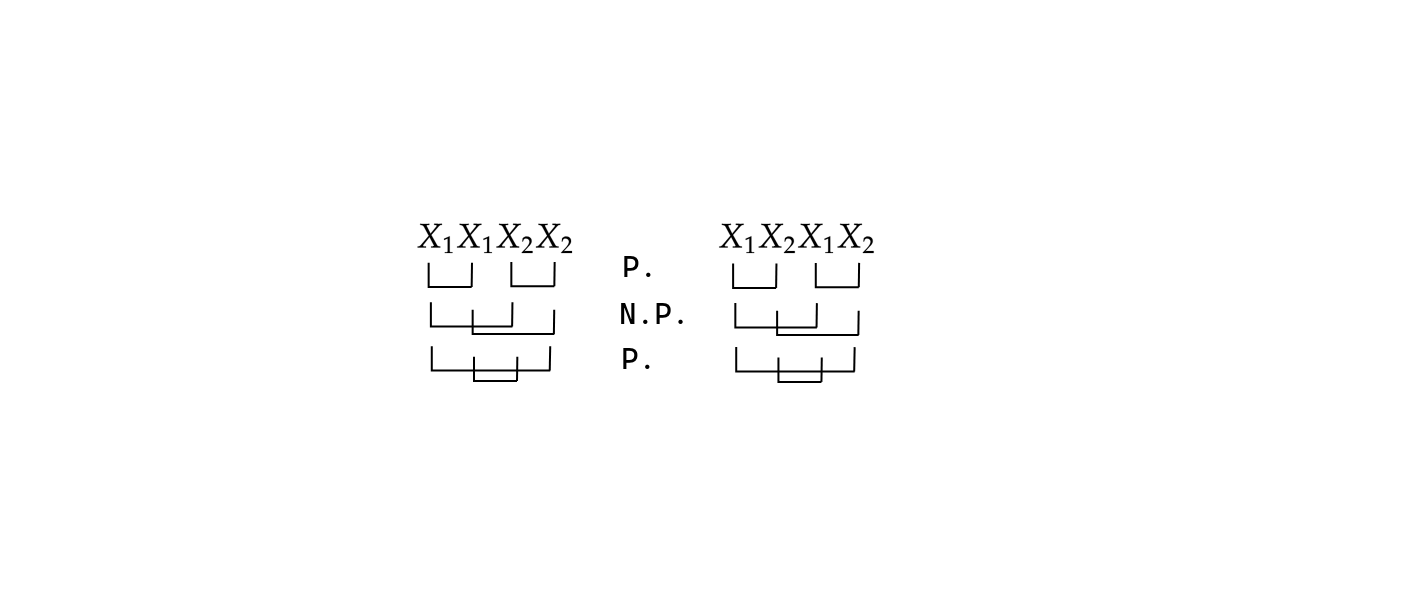
\includegraphics[width=\linewidth]{figures/contractions.png}\\
      {\footnotesize Planar (P.) and Non-Planar (N.P.) contractions of the quartic interaction.}
    \end{column}
    \begin{column}{0.54\textwidth}
      \footnotesize
      The interaction $\tfrac{\lambda}{2}\big(\Tr X_1X_1X_2X_2-\Tr X_1X_2X_1X_2\big)$ gives two channels:
      \begin{itemize}
        \item \hl{Planar:} clean factorization
          \begin{equation*}
            \mathcal{K}^{l_1 l_1 l_2 l_2}\sigma_{xx}(l_1)\sigma_{xx}(l_2)
              =\tfrac{1}{N}\,C^2.
          \end{equation*}
        \item \new{Non-planar:} brings in the $6j$-symbol
          \begin{equation*}
            G(l_1,l_2)=(-1)^{\cdots}\sixj{l_1}{\!\frac{N-1}{2}\!}{\!\frac{N-1}{2}\!}{l_2}{\!\frac{N-1}{2}\!}{\!\frac{N-1}{2}\!}.
          \end{equation*}
      \end{itemize}
      \new{Crucial point:} because the symmetry is $SU(2)$ (not $SU(N)$), the non-planar term is \hl{not} $1/N^2$-suppressed!
    \end{column}
  \end{columns}
\end{frame}

\begin{frame}{Equation of State: Self-Consistency}
  Entropy maximization at fixed energy ($\mathcal{L}=S-\beta(E-E_{eq})$) gives the thermal ratio
  \begin{equation*}
    \frac{\sigma_{pp}(l)}{\sigma_{xx}(l)}=\omega_l^2,\qquad
    f_l=\tfrac{1}{2}\coth\!\big(\tfrac{\beta\omega_l}{2}\big),\qquad \beta=1/T.
  \end{equation*}
  \begin{columns}[T]
    \begin{column}{0.5\textwidth}
      \begin{block}{Planar}
        Single self-consistency equation for $C$:
        \begin{equation*}
          \omega_l=\sqrt{\mu^2+\tfrac{l(l+1)}{R^2}+\tfrac{\lambda C}{N}}.
        \end{equation*}
      \end{block}
    \end{column}
    \begin{column}{0.5\textwidth}
      \begin{block}{\new{Full (non-planar)}}
        $N$ coupled equations via $D(l)=\sum_{l'}(2l'+1)\sigma_{xx}(l')G(l,l')$:
        \begin{equation*}
          \omega_l=\sqrt{\mu^2+\tfrac{l(l+1)}{R^2}+\tfrac{\lambda C}{N}-\lambda D(l)}.
        \end{equation*}
      \end{block}
    \end{column}
  \end{columns}
  \vspace{0.4em}
  \begin{equation*}
    \sigma_{xx}(l)=\frac{1}{2\omega_l[\vec\sigma]}\coth\!\Big(\frac{\beta\,\omega_l[\vec\sigma]}{2}\Big),
    \quad l=0,\dots,N-1 \quad\text{(solved numerically).}
  \end{equation*}
\end{frame}

\begin{frame}{Energy \& Coordinate Dispersion vs.\ Temperature \newflag}
  \begin{figure}
    \captionsetup[subfigure]{skip=-7pt}   % ← default is ~10pt
    \centering
    \begin{subfigure}[b]{0.35\textwidth}
      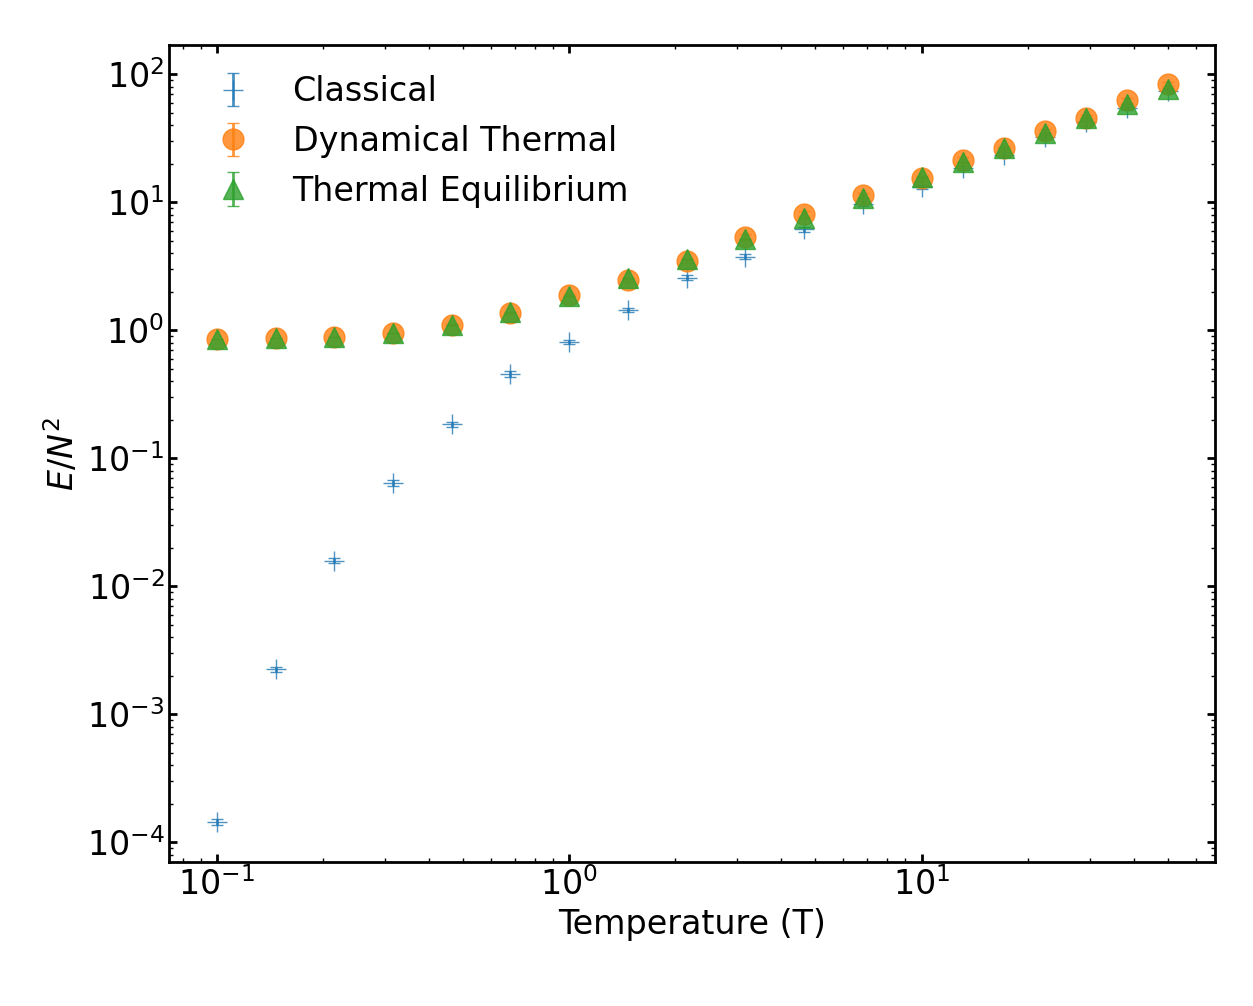
\includegraphics[width=\linewidth]{figures/EnergyVsTPlanarAll.png}
      \caption*{\scriptsize $E/N^2$ -- Planar}
    \end{subfigure}\hfil
    \begin{subfigure}[b]{0.35\textwidth}
      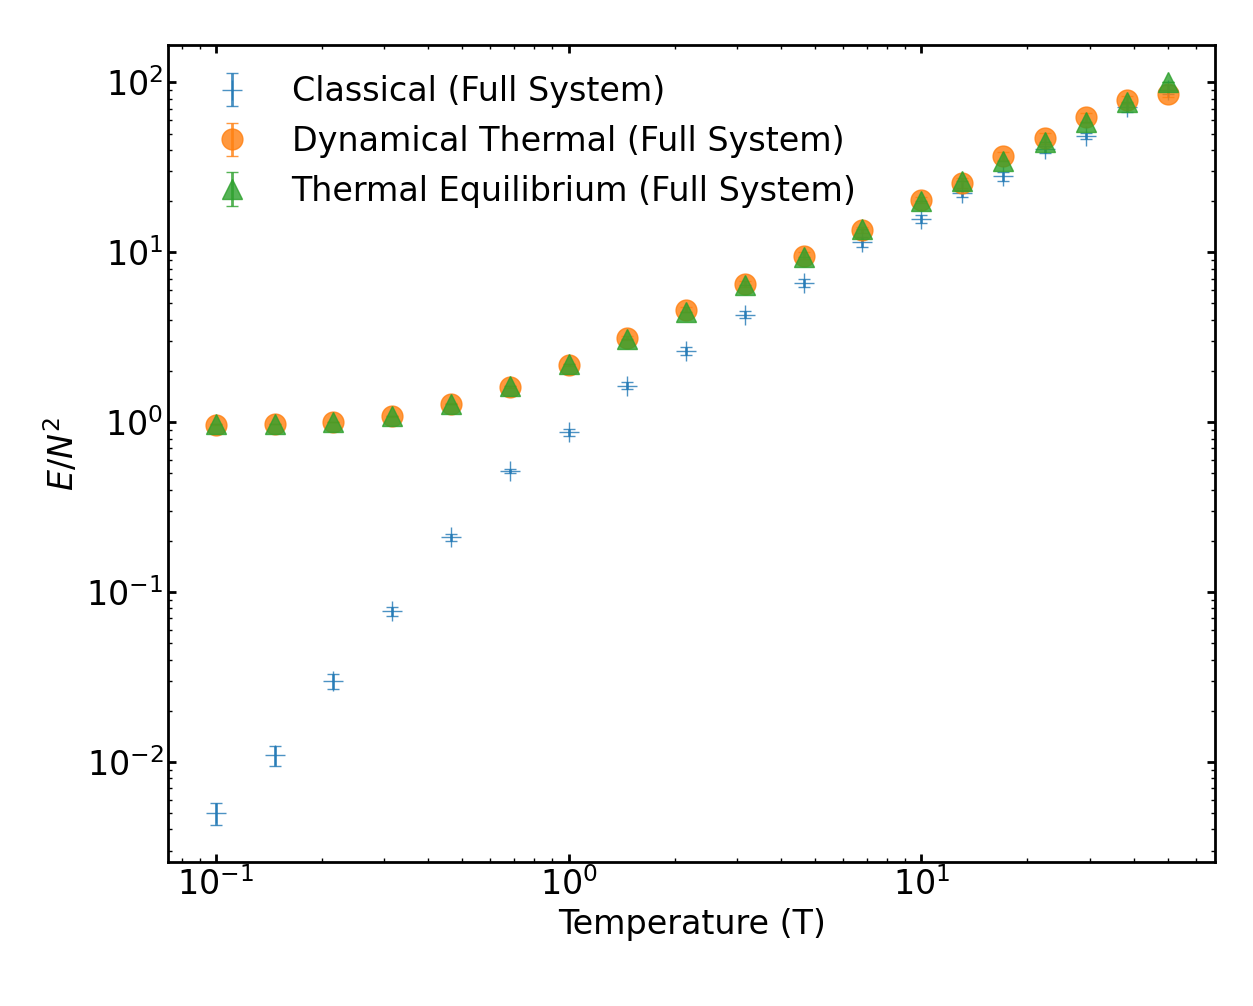
\includegraphics[width=\linewidth]{figures/EnergyVsTNonPlanarAll.png}
      \caption*{\scriptsize $E/N^2$ -- \new{Full}}
    \end{subfigure}\\[-0.8em]
    \begin{subfigure}[b]{0.35\textwidth}
      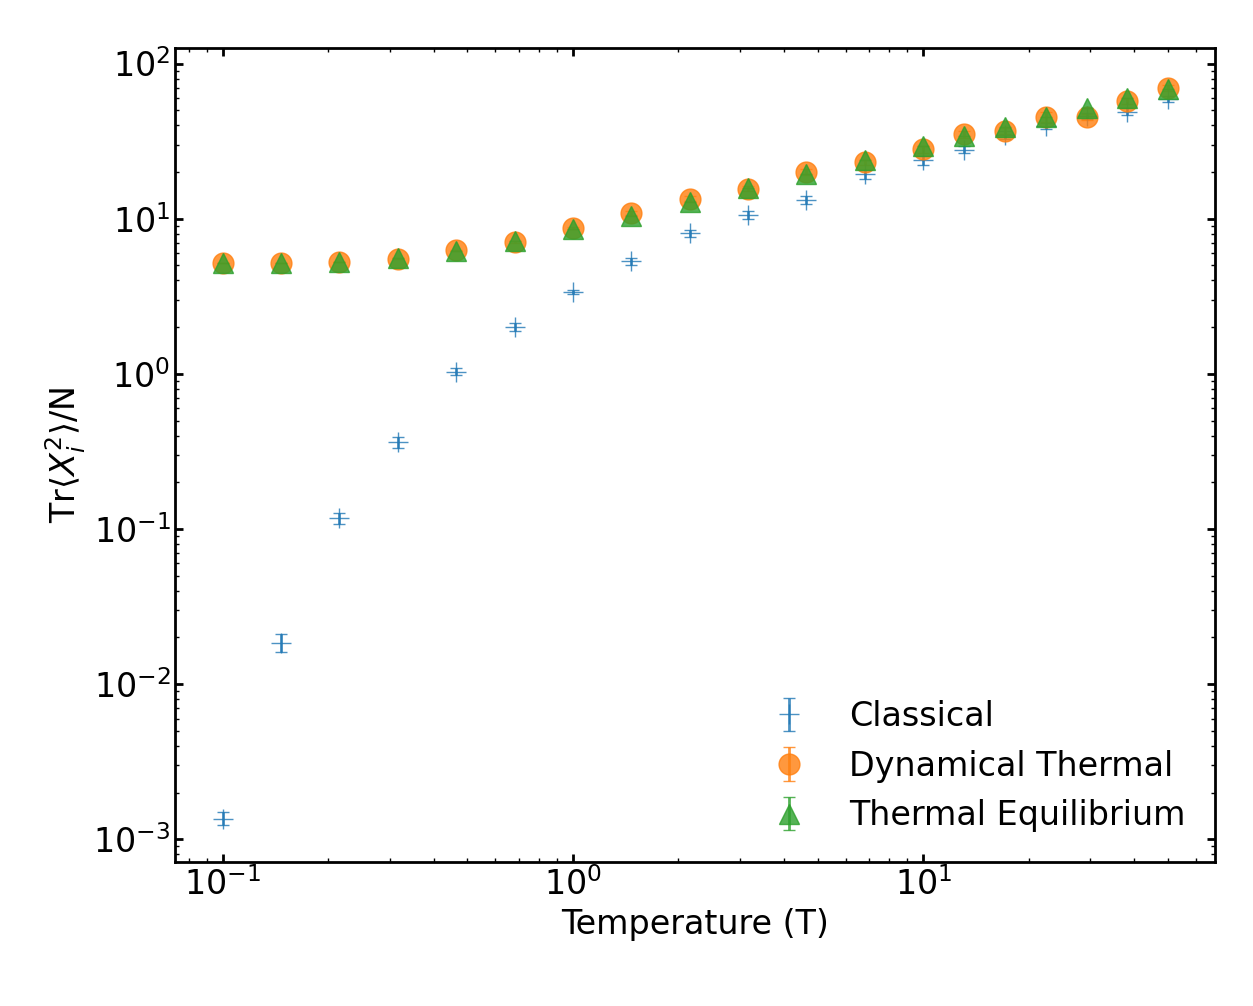
\includegraphics[width=\linewidth]{figures/TraceVsTPlanarAll.png}
      \caption*{\scriptsize $\tfrac{1}{N}\dbk{\Tr X_iX_i}$ -- Planar}
    \end{subfigure}\hfil
    \begin{subfigure}[b]{0.35\textwidth}
      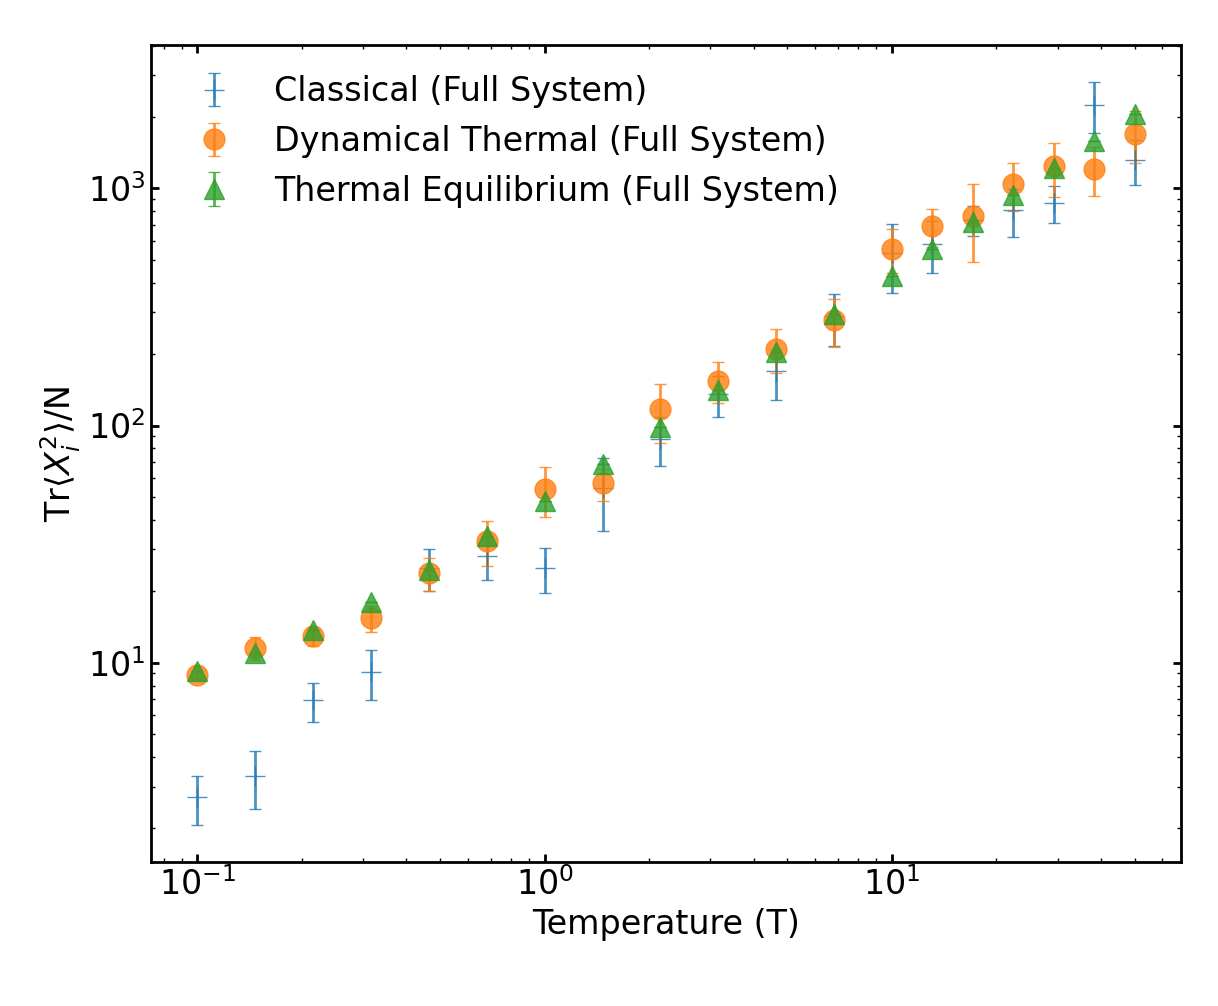
\includegraphics[width=\linewidth]{figures/TraceVsTNonPlanarAll.png}
      \caption*{\scriptsize $\tfrac{1}{N}\dbk{\Tr X_iX_i}$ -- \new{Full}}
    \end{subfigure}
  \end{figure}
  \vspace{-1.4em}
\end{frame}

\begin{frame}{\new{Entropy} \& \new{the Bekenstein Bound} \newflag}
  \begin{columns}[T]
    \begin{column}{0.5\textwidth}
      \centering
      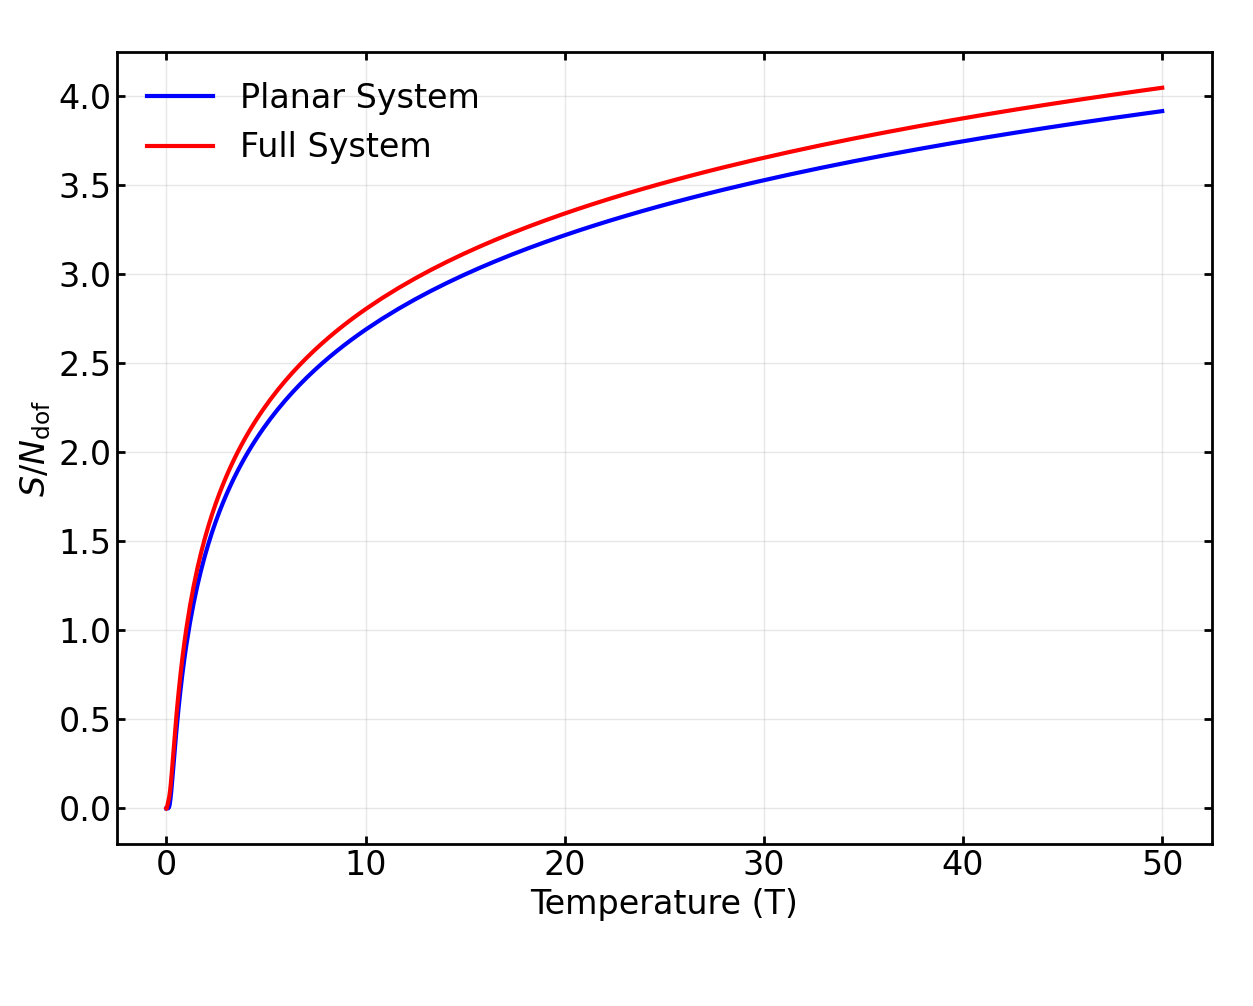
\includegraphics[width=\linewidth]{figures/EntropyVsT.png}\\
      {\scriptsize $S/N_{\mathrm{dof}}$ vs $T$ \ ($N_{\mathrm{dof}}=2N^2=50$).}
    \end{column}
    \begin{column}{0.5\textwidth}
      \centering
      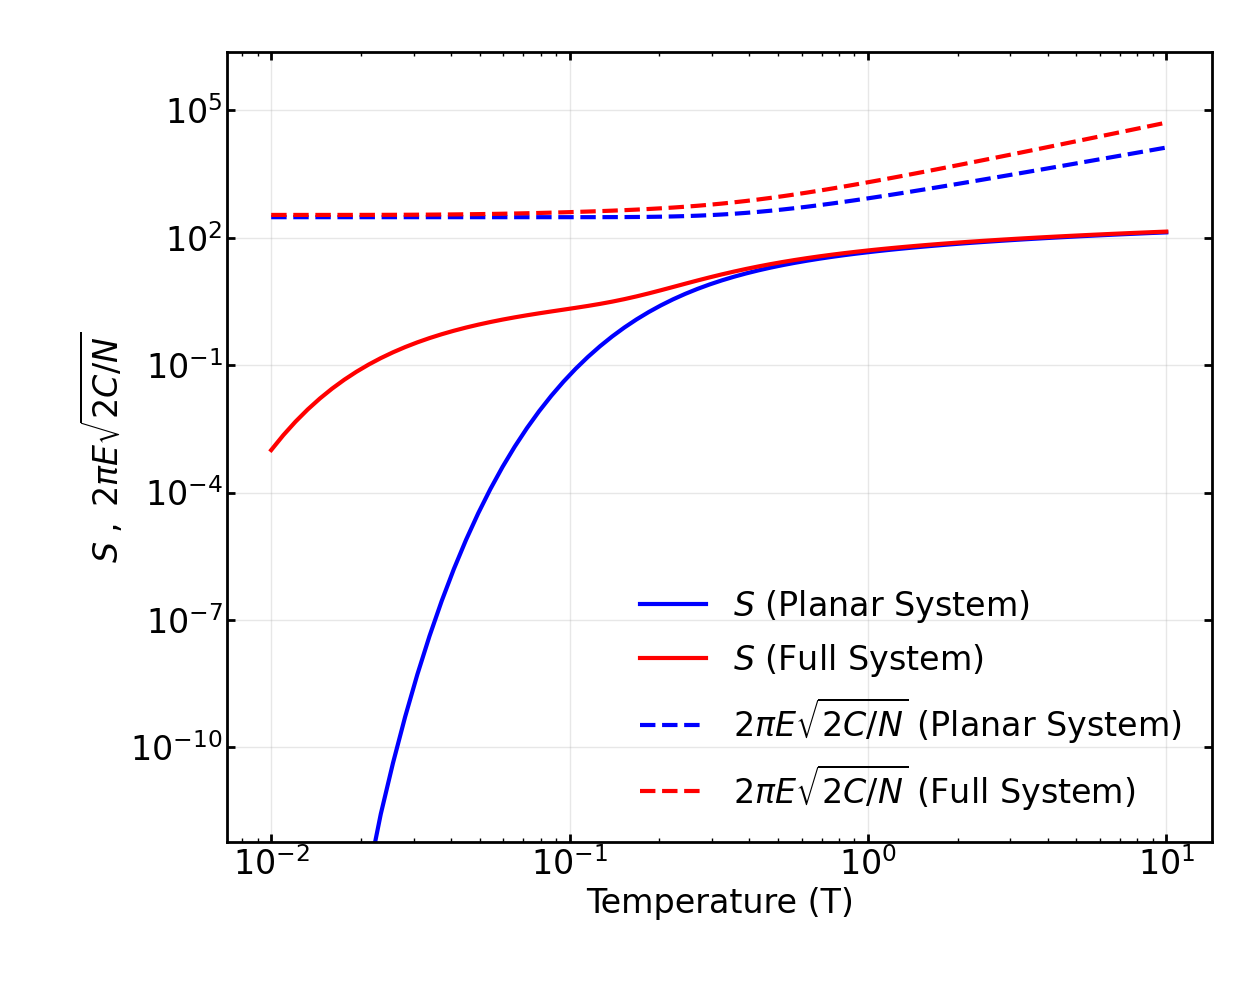
\includegraphics[width=\linewidth]{figures/EntropyVsTPlanarNonPlanar.png}\\
      {\scriptsize $S$ vs the bound $2\pi E\sqrt{2C/N}$.}
    \end{column}
  \end{columns}
  \vspace{0.3em}
  \begin{itemize}\footnotesize
    \item Entropy increases monotonically with $T$; the small dent (full, red) near $T\approx 0.1$ is the decoupled $l=0$ mode.
    \item \hl{Bekenstein bound} $S\le 2\pi E K$ with $K=\sqrt{\tfrac{1}{N}\dbk{\Tr X_iX_i}}$ is comfortably satisfied: $S\ll 2\pi E\sqrt{2C/N}$.
  \end{itemize}
\end{frame}

\begin{frame}{Choosing Dynamical Initial Conditions}
  \begin{alertblock}{The problem}
    The thermal state is a \emph{static} solution of the EOM $\Rightarrow$ no chaos from small fluctuations.
  \end{alertblock}
  \textbf{Solution:} split each dispersion into quantum + classical parts,
  \begin{equation*}
    \sigma_{\xi\xi}(l)=\sigma^0_{\xi\xi}(l)+\sigma^c_{\xi\xi}(l),
  \end{equation*}
  \begin{itemize}
    \item $\sigma^0$: zero-temperature (pure-state) quantum dispersion.
    \item $\sigma^c$: classical thermal dispersion (difference from $T=0$).
  \end{itemize}
  Build a classical mixture of \hl{shifted pure Gaussian states} $\ket{\bar X_i^{lm},\bar P_i^{lm}}$ with 1-point functions drawn randomly from Gaussians of variance $\sigma^c$. This \new{dynamical thermal state} is time-dependent, sits on the thermal equation of state, and encodes the chaotic motion.
\end{frame}

\begin{frame}{Dynamical Thermal States Track Equilibrium \newflag}
  \begin{figure}
    \captionsetup[subfigure]{skip=-14pt}   % ← default is ~10pt
    \centering
    \begin{subfigure}[b]{0.35\textwidth}
      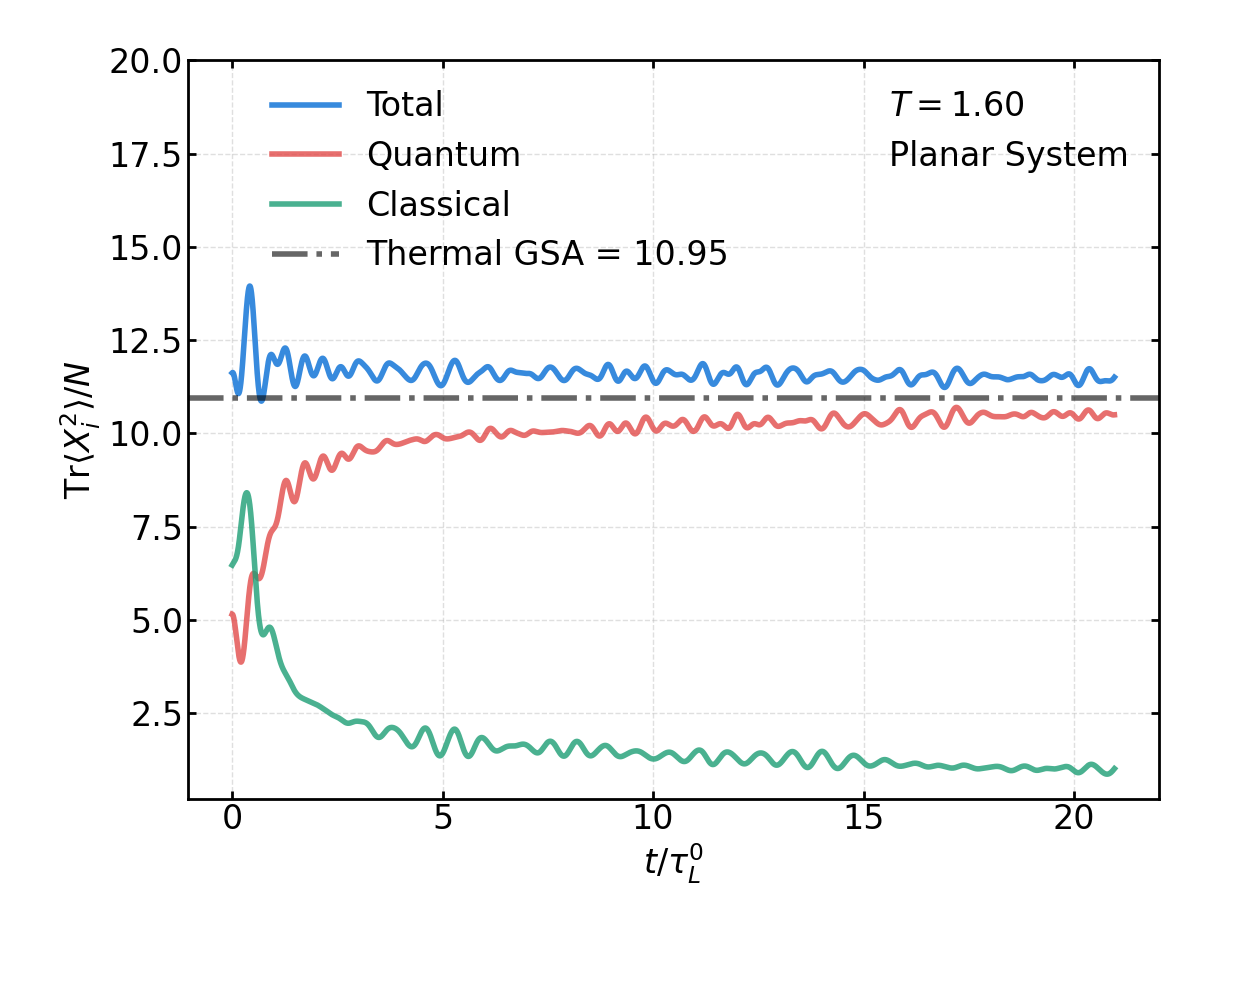
\includegraphics[width=\linewidth]{figures/TraceVsTimeT1.6Planar.png}
      \caption*{\scriptsize Planar, $T=1.6$}
    \end{subfigure}\hfil
    \begin{subfigure}[b]{0.35\textwidth}
      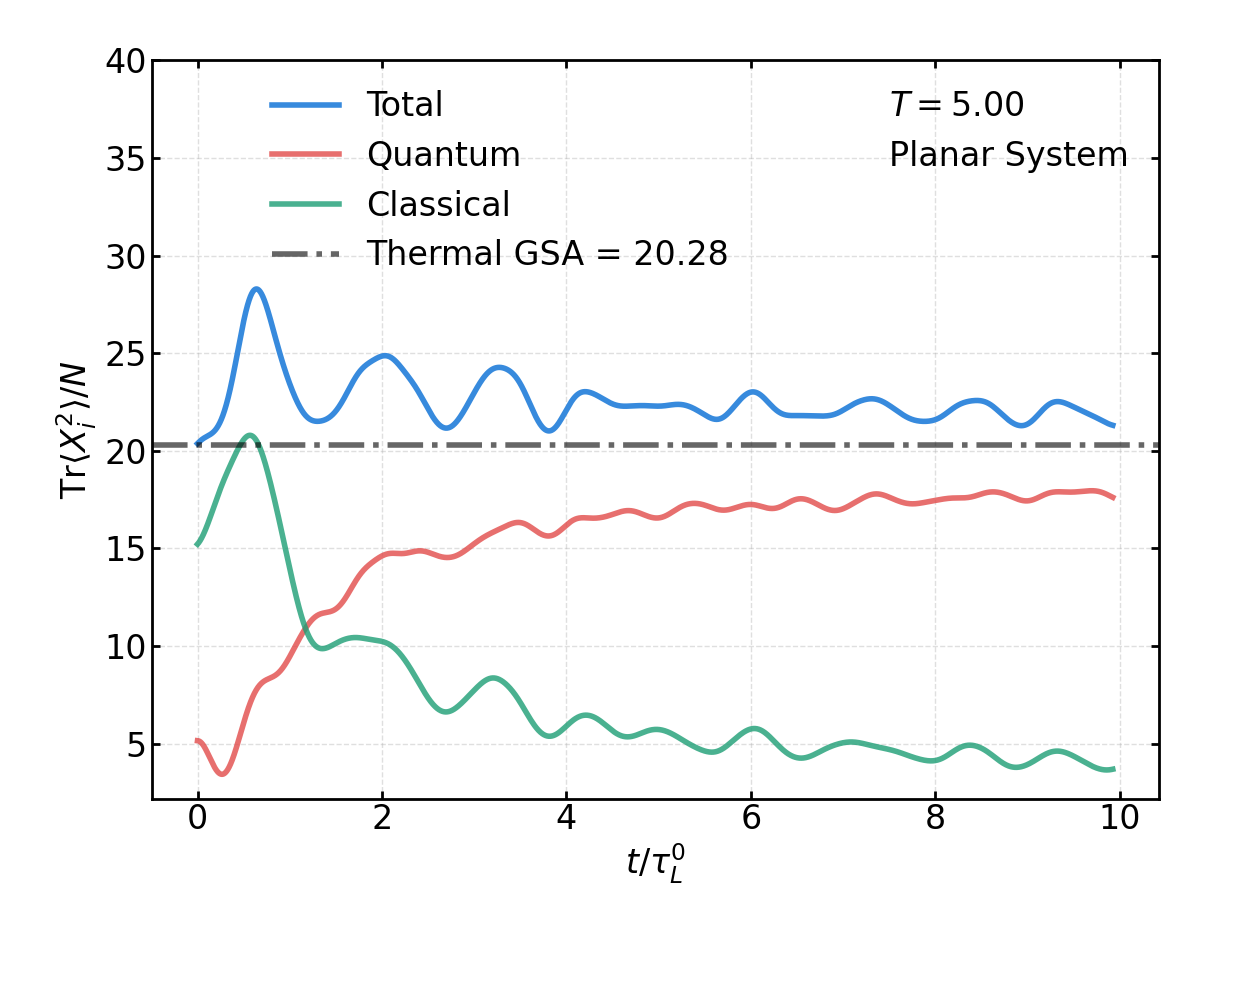
\includegraphics[width=\linewidth]{figures/TraceVsTimeT5Planar.png}
      \caption*{\scriptsize Planar, $T=5$}
    \end{subfigure}\\[-0.8em]
    \begin{subfigure}[b]{0.35\textwidth}
      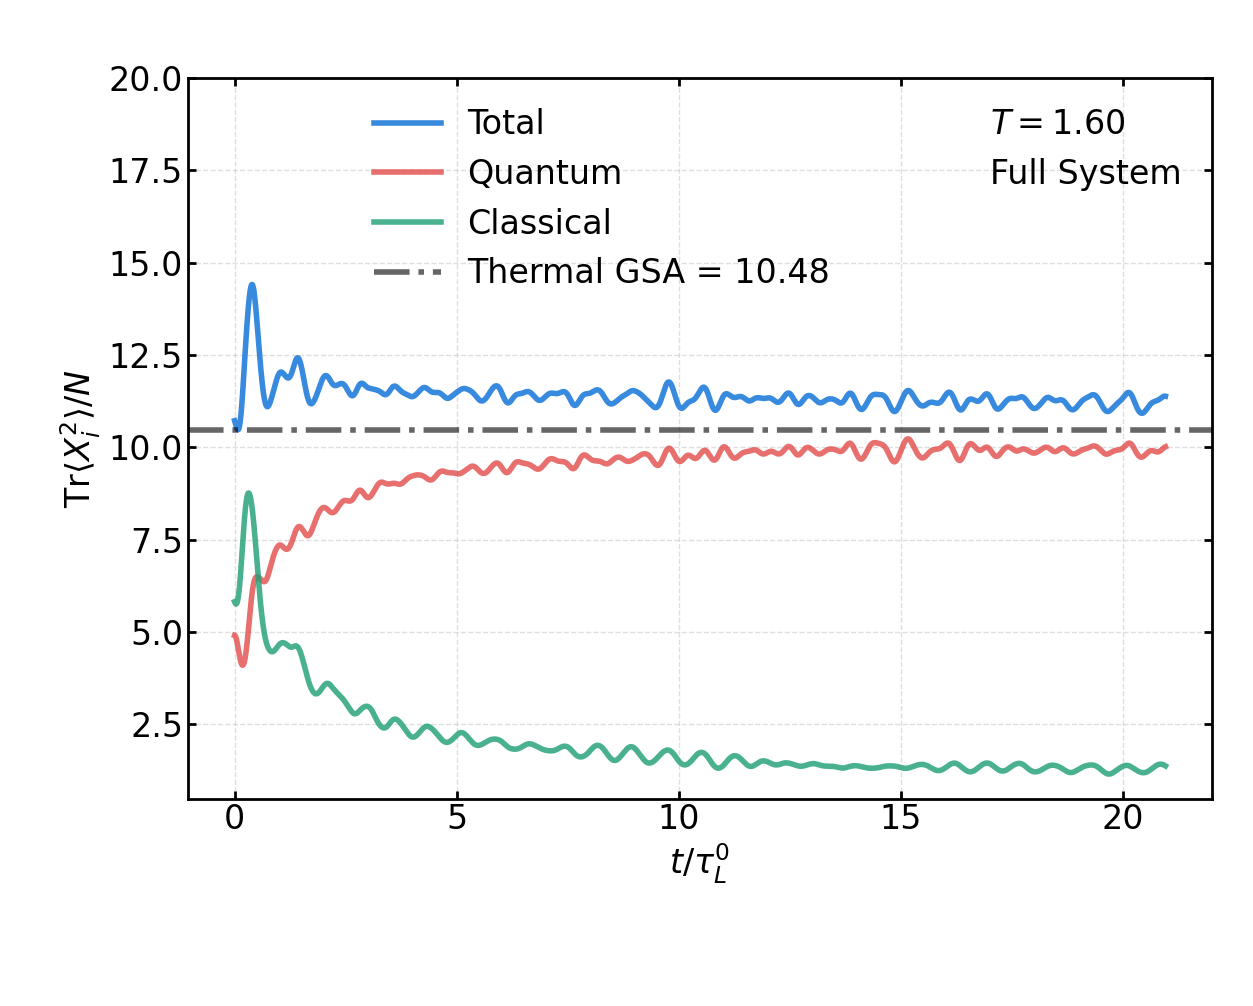
\includegraphics[width=\linewidth]{figures/TraceVsTimeT1.6NonPlanar.png}
      \caption*{\scriptsize \new{Full}, $T=1.6$}
    \end{subfigure}\hfil
    \begin{subfigure}[b]{0.35\textwidth}
      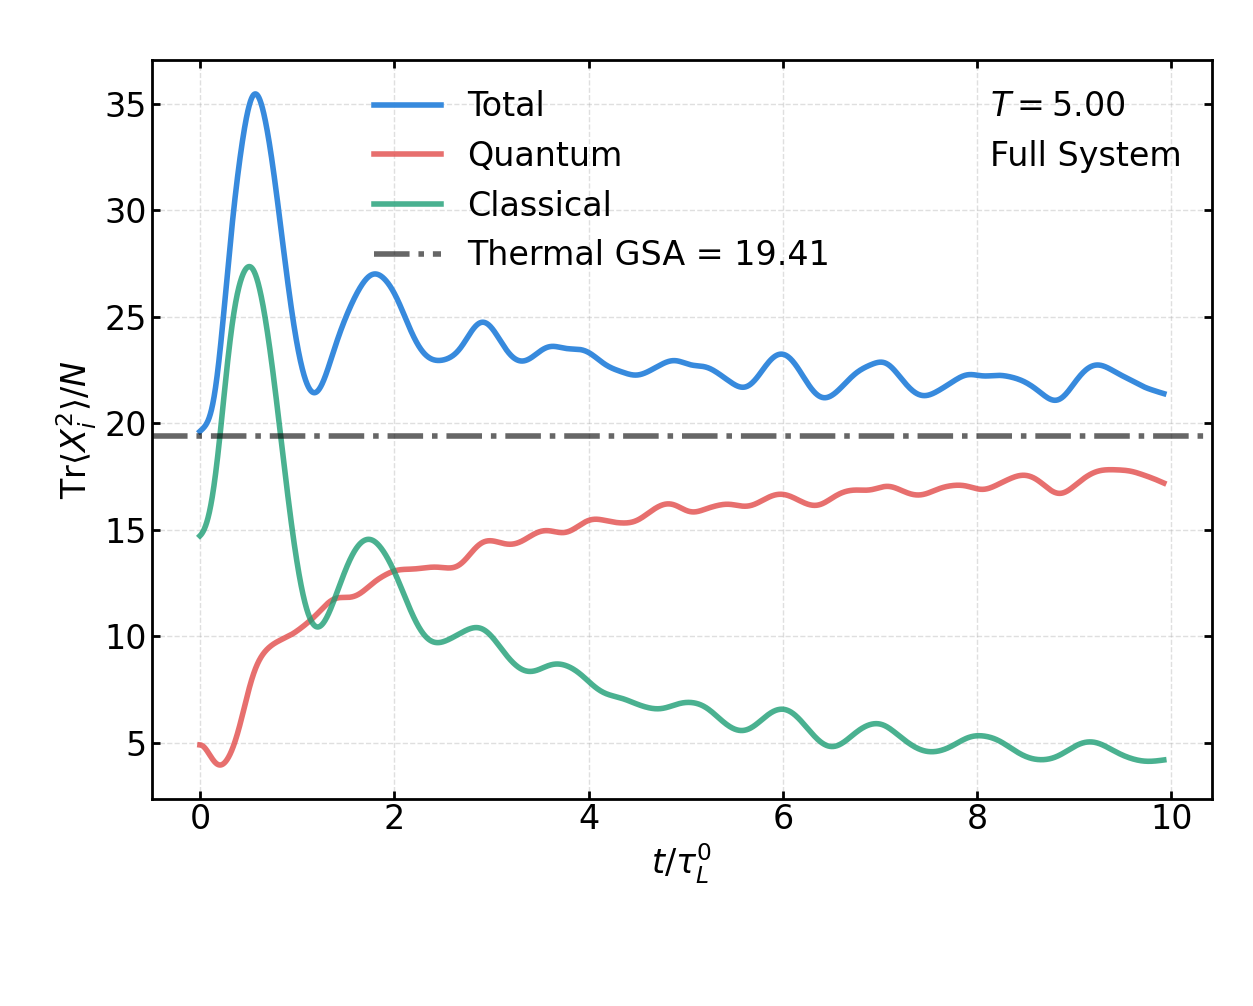
\includegraphics[width=\linewidth]{figures/TraceVsTimeT5NonPlanar.png}
      \caption*{\scriptsize \new{Full}, $T=5$}
    \end{subfigure}
  \end{figure}
  \vspace{-1.8em}
  {\footnotesize $\tfrac{1}{N}\dbk{\Tr XX}$ vs time (units of $\tau_L=\lambda_L^{-1}$). It fluctuates with small amplitude just above its equilibrium value.}
\end{frame}

% ==============================================================
% Section 4: Dynamics, Chaos & Results
% ==============================================================
\section{Dynamics}

\begin{frame}{Computing the Largest Lyapunov Exponent}
  \begin{columns}[T]
    \begin{column}{0.58\textwidth}
      \centering
      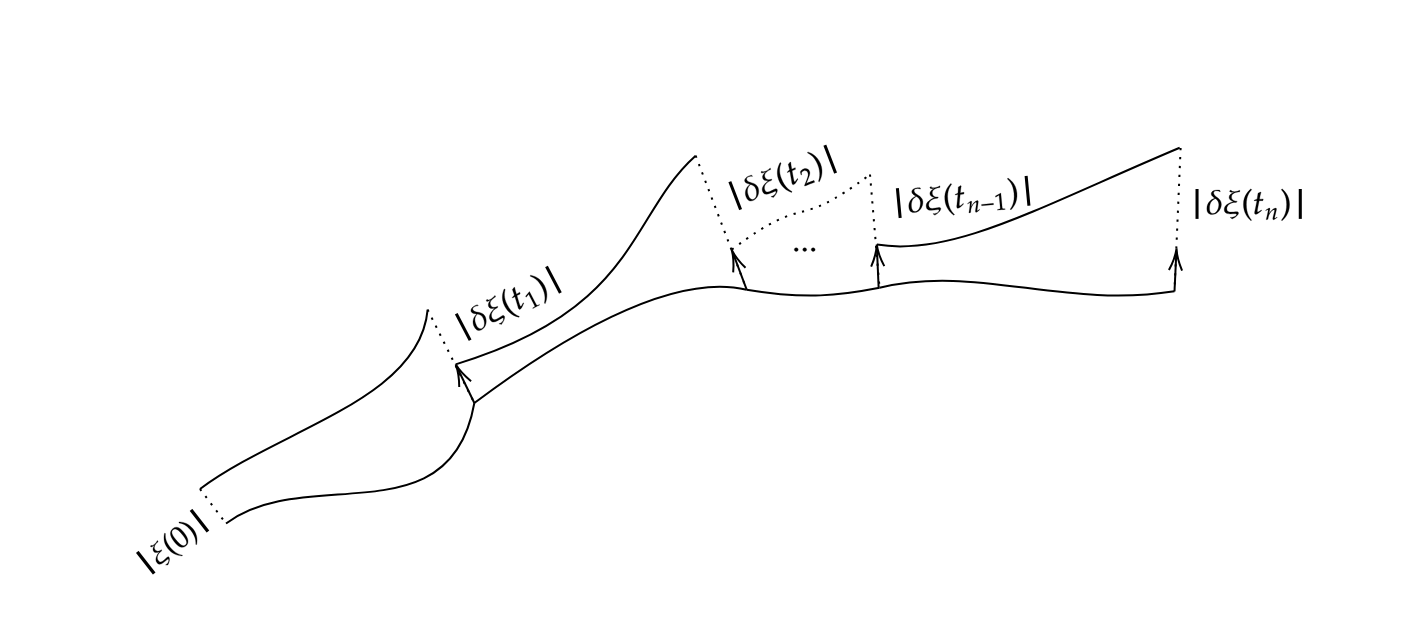
\includegraphics[width=\linewidth]{figures/lyapunov-exponents.png}\\
      {\scriptsize Renormalize-and-sum procedure for $\lambda_L$.}
    \end{column}
    \begin{column}{0.42\textwidth}
      \begin{itemize}\small
        \item Integrate two nearby trajectories, $\|\delta\xi(0)\|\approx 10^{-5}$.
        \item Measure separation, renormalize, accumulate growth.
        \item Average over 7--9 random initial conditions.
      \end{itemize}
    \end{column}
  \end{columns}
  \vspace{0.4em}
  \begin{equation*}
    \lambda_L=\lim_{t\to\infty}\frac{1}{t}\ln\frac{\|\delta\xi(t)\|}{\|\delta\xi(0)\|}
      \;\longrightarrow\;
      \lambda_L\approx\frac{1}{n\Delta t}\sum_{i=1}^{n}\ln\frac{\|\delta\xi(t_i)\|}{\|\delta\xi(0)\|}.
  \end{equation*}
  {\footnotesize \textbf{Implementation:} C++ code, \hl{symplectic Euler} integrator (update order $P\to XP\to PP\to XX\to X$), run on the TRUBA HPC cluster with SLURM job arrays.}
\end{frame}

\begin{frame}{$\lambda_L$ Time Series: Transient $\to$ Saturation \newflag}
  \begin{figure}
    \captionsetup[subfigure]{skip=-18pt}   % ← default is ~10pt
    \centering
    \begin{subfigure}[b]{0.35\textwidth}
      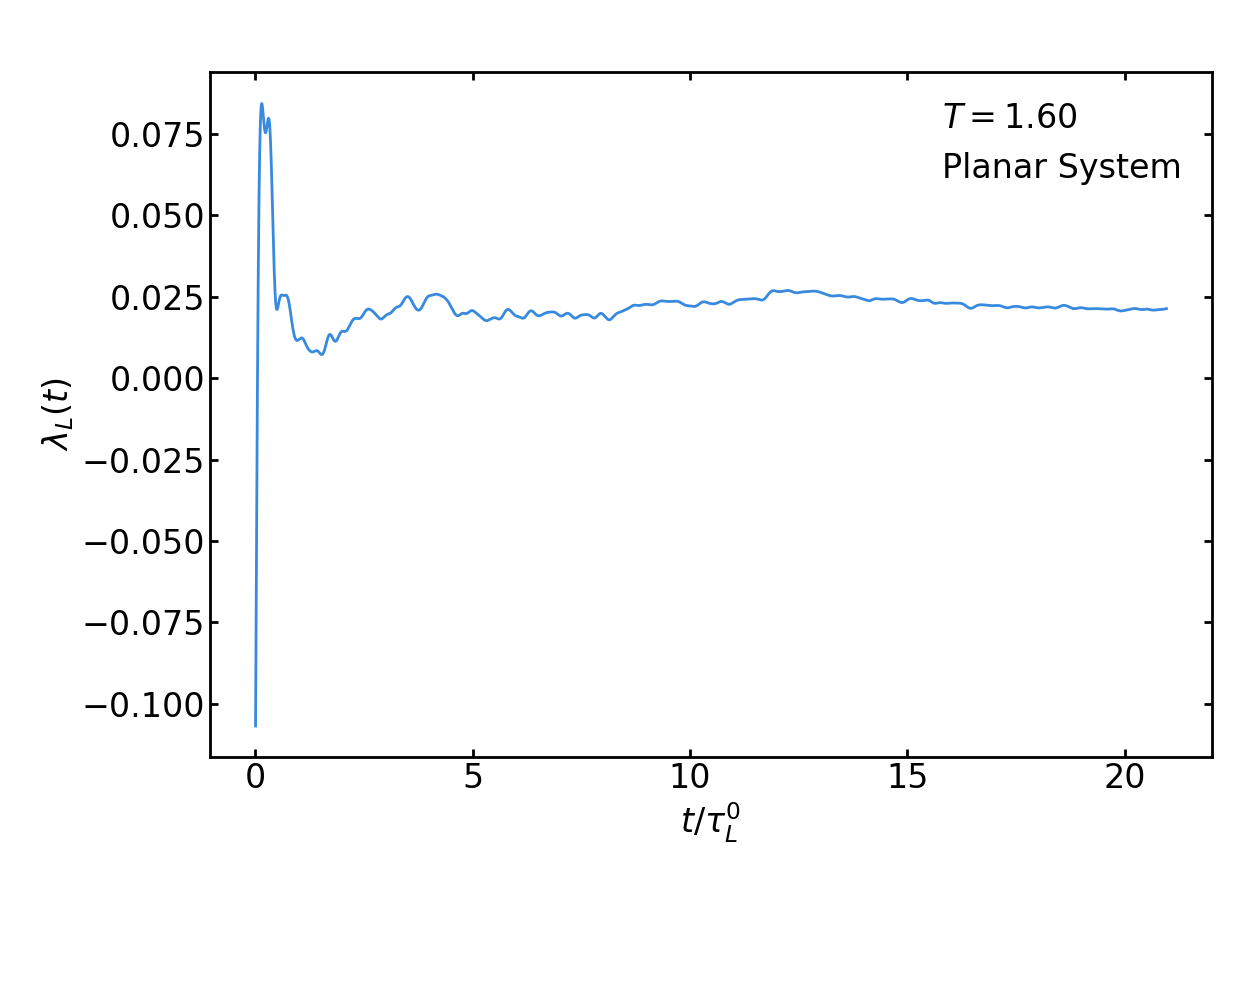
\includegraphics[width=\linewidth]{figures/LyapTimePlanarT16.png}
      \caption*{\scriptsize Planar, $T=1.6$}
    \end{subfigure}\hfil
    \begin{subfigure}[b]{0.35\textwidth}
      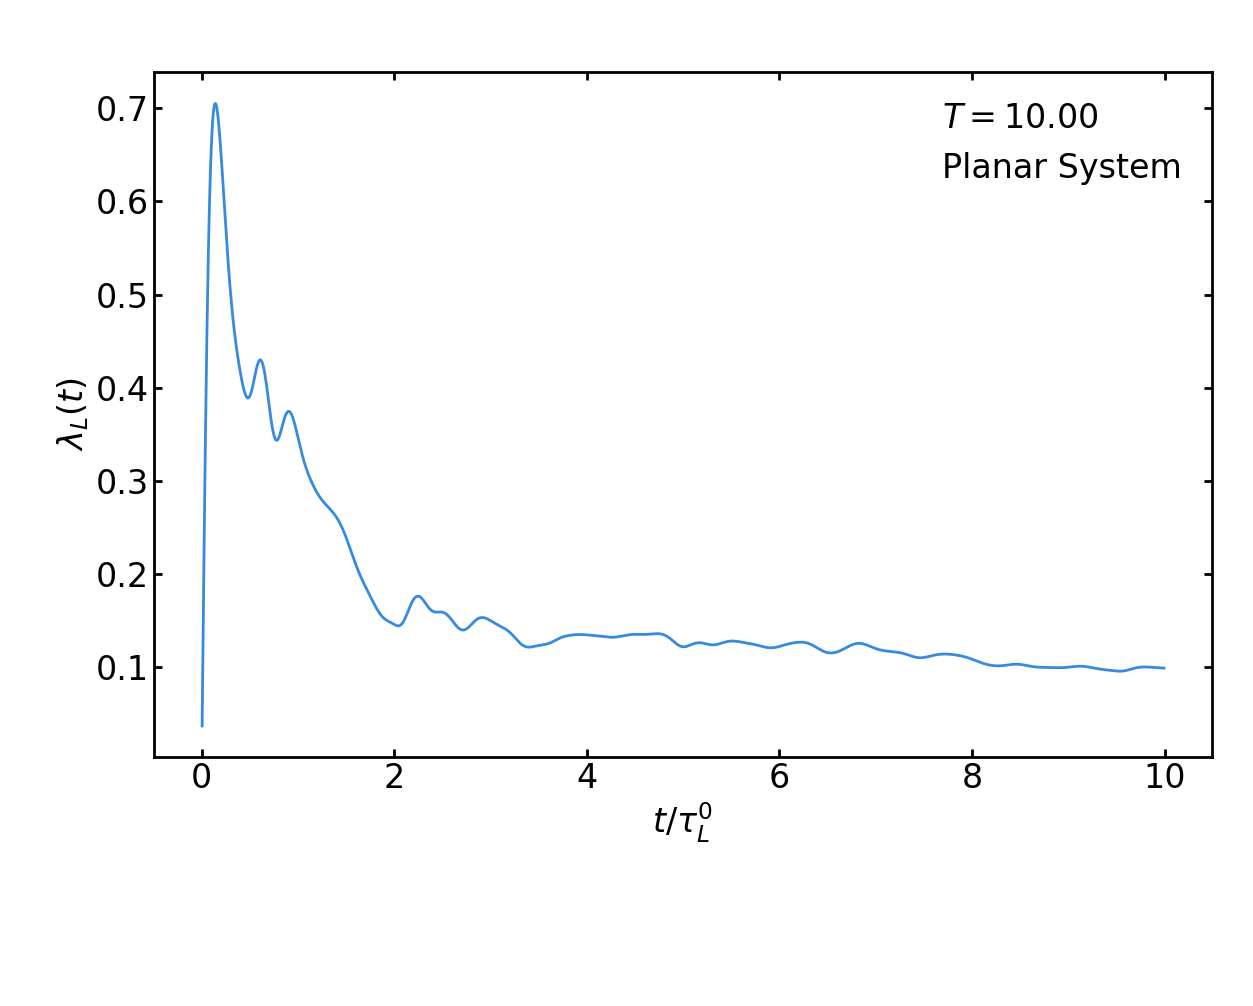
\includegraphics[width=\linewidth]{figures/LyapTimePlanarT10.png}
      \caption*{\scriptsize Planar, $T=10$}
    \end{subfigure}\\[-0.9em]
    \begin{subfigure}[b]{0.35\textwidth}
      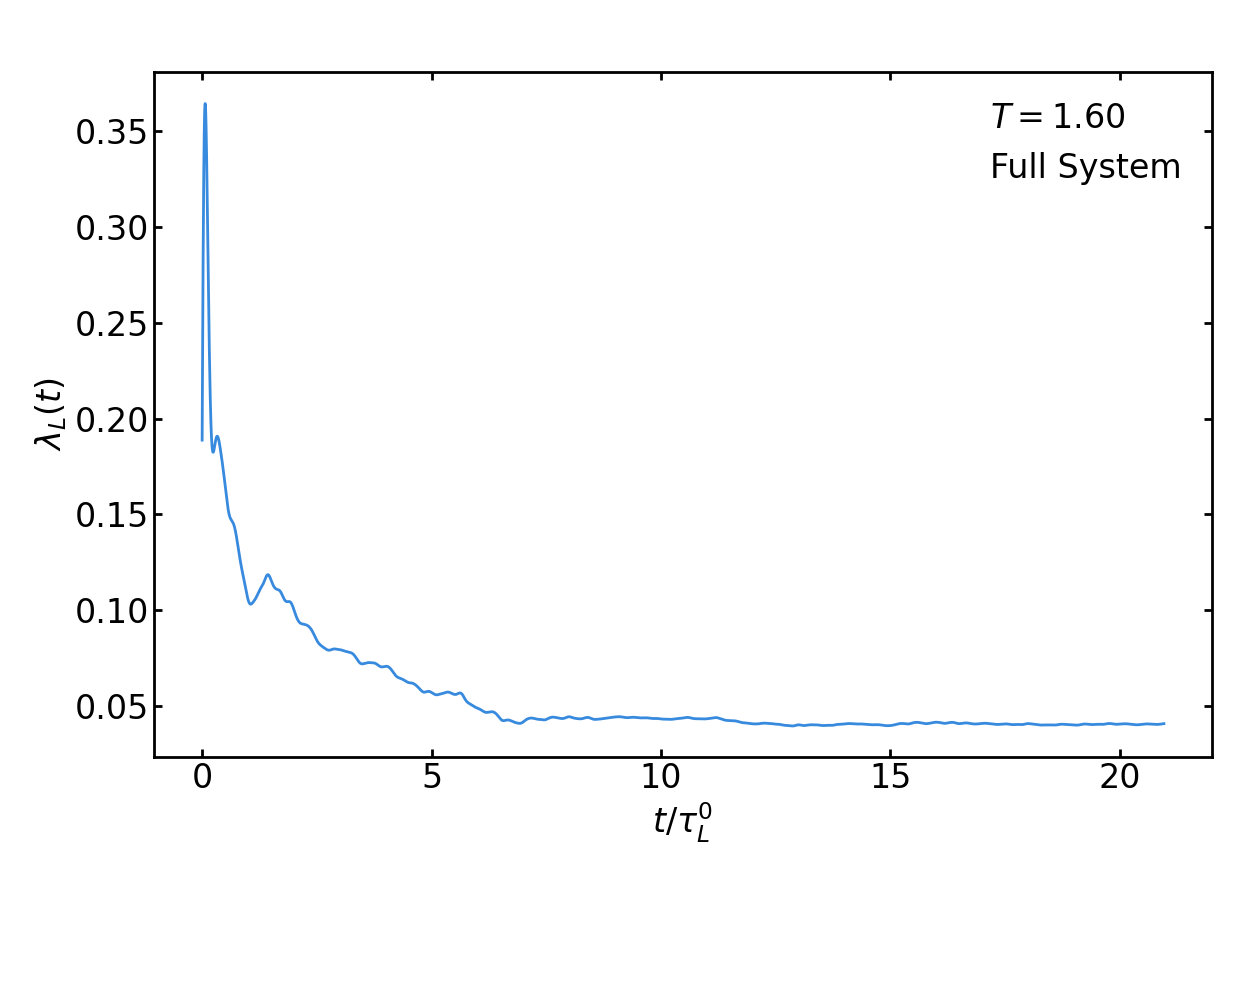
\includegraphics[width=\linewidth]{figures/LyapTimeNonPlanarT16.png}
      \caption*{\scriptsize \new{Full}, $T=1.6$}
    \end{subfigure}\hfil
    \begin{subfigure}[b]{0.35\textwidth}
      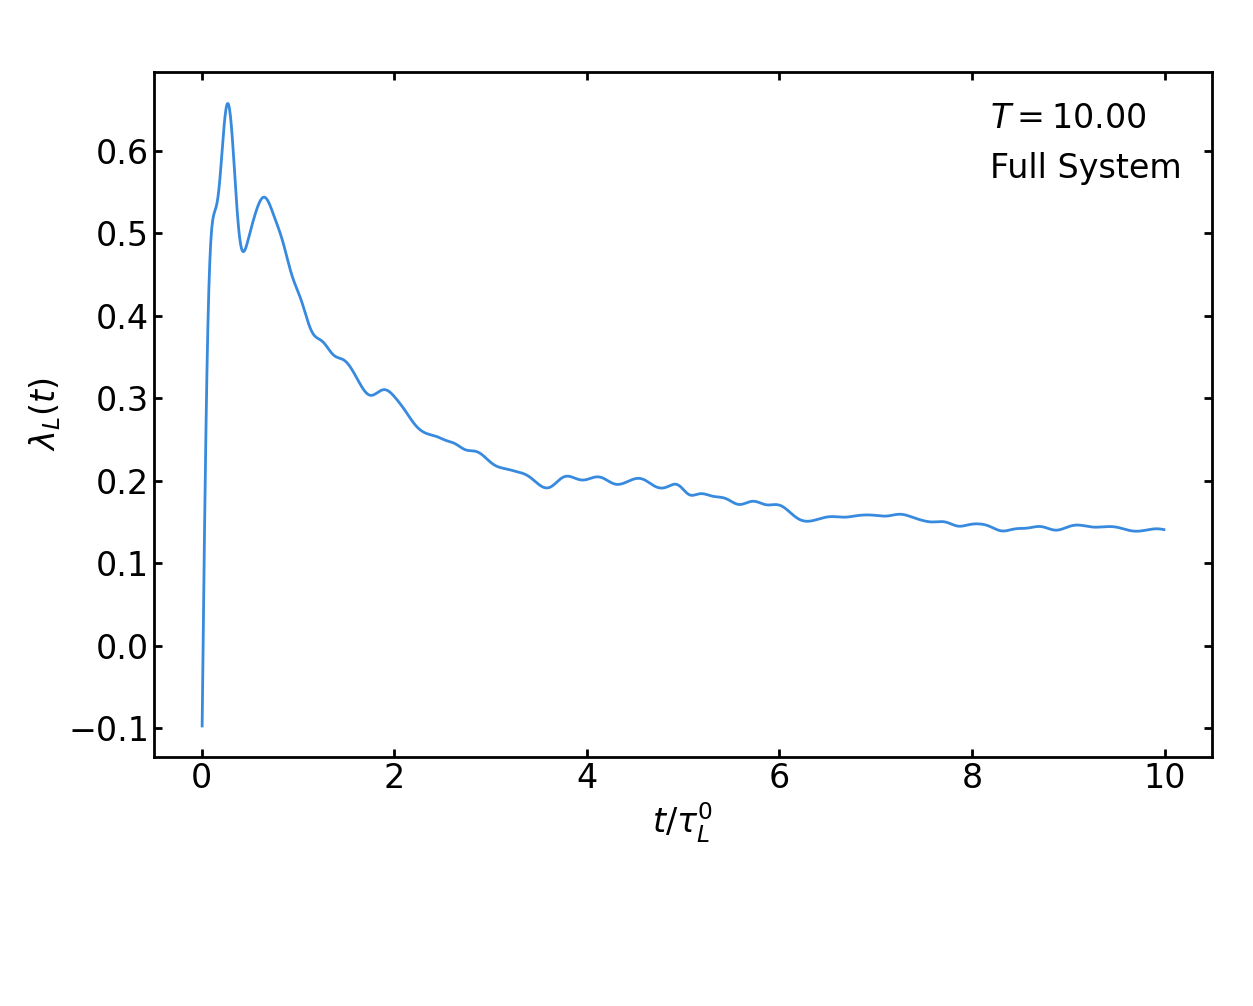
\includegraphics[width=\linewidth]{figures/LyapTimeNonPlanarT10.png}
      \caption*{\scriptsize \new{Full}, $T=10$}
    \end{subfigure}
  \end{figure}
  \vspace{-0.8em}
  {\footnotesize After a transient within the first $\sim 2\tau_L^{(0)}$ (planar) / $\sim 6\tau_L^{(0)}$ (full), $\lambda_L$ converges to a stable saturation value.}
\end{frame}

\begin{frame}{Main Result: $\lambda_L$ vs.\ Temperature \& the MSS Bound \newflag}
  \begin{columns}[c]
    \begin{column}{0.6\textwidth}
      \centering
      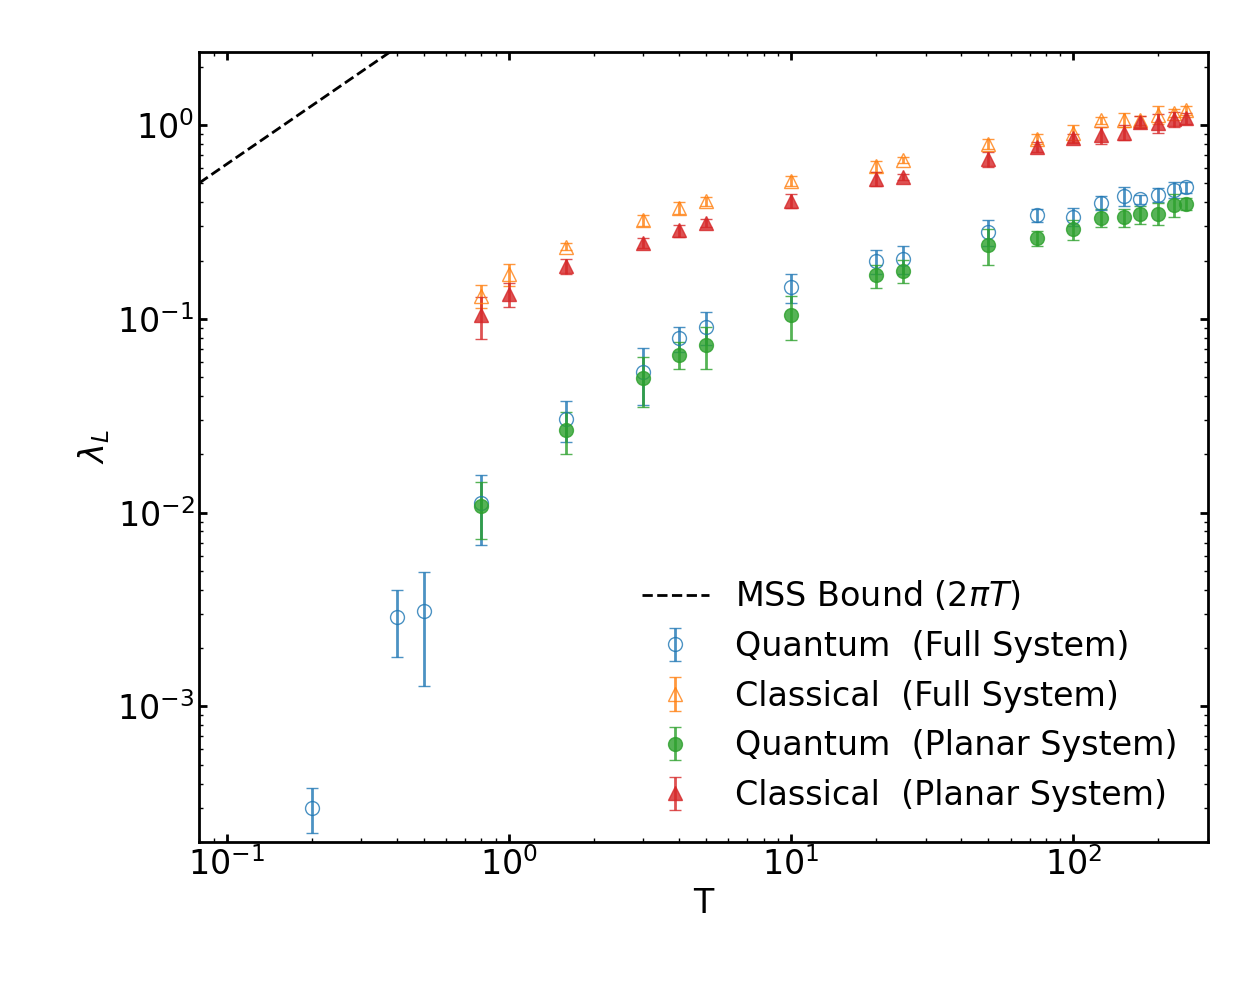
\includegraphics[width=\linewidth]{figures/LyapunovVsTPlanarNonPlanar2.png}
    \end{column}
    \begin{column}{0.4\textwidth}
      \footnotesize
      \begin{itemize}
        \item \hl{MSS bound $\lambda_L\le 2\pi T$ respected at all $T$.}
        \item $\lambda_L\to 0$ at finite $T_c$: \new{quantum effects suppress chaos} as $T$ drops.
        \begin{itemize}\scriptsize
          \item Planar: $T_c\lesssim 0.8$
          \item Full: $T_c\approx 0.1$
        \end{itemize}
        \item Quantum $\to$ classical as $T\gtrsim 10^2$, always staying below.
        \item Full system slightly more chaotic than planar everywhere.
      \end{itemize}
    \end{column}
  \end{columns}
  \vspace{0.3em}
  {\footnotesize $N=5,\ R=5,\ \mu=1/10,\ \lambda=1/5$. This plot is the central physics result of the completed bosonic work.}
\end{frame}

\begin{frame}{$N$-dependence and Curvature ($R$) dependence \newflag}
  \begin{columns}[T]
    \begin{column}{0.33\textwidth}
      \centering
      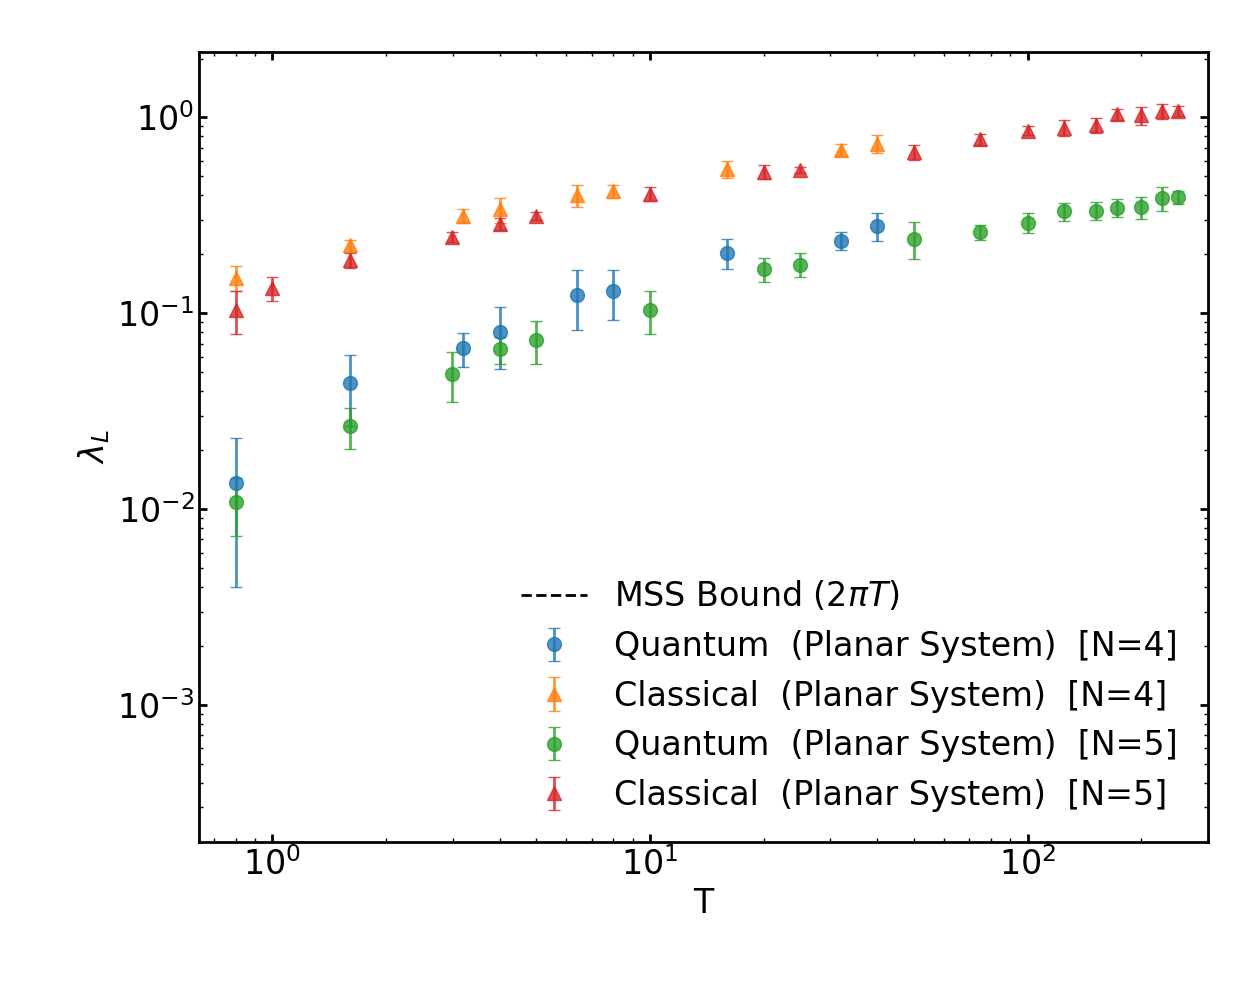
\includegraphics[width=\linewidth]{figures/LyapunovVsTPlanarN4N51.png}\\
      {\scriptsize Planar: $N=4$ vs $N=5$.}
    \end{column}
    \begin{column}{0.33\textwidth}
      \centering
      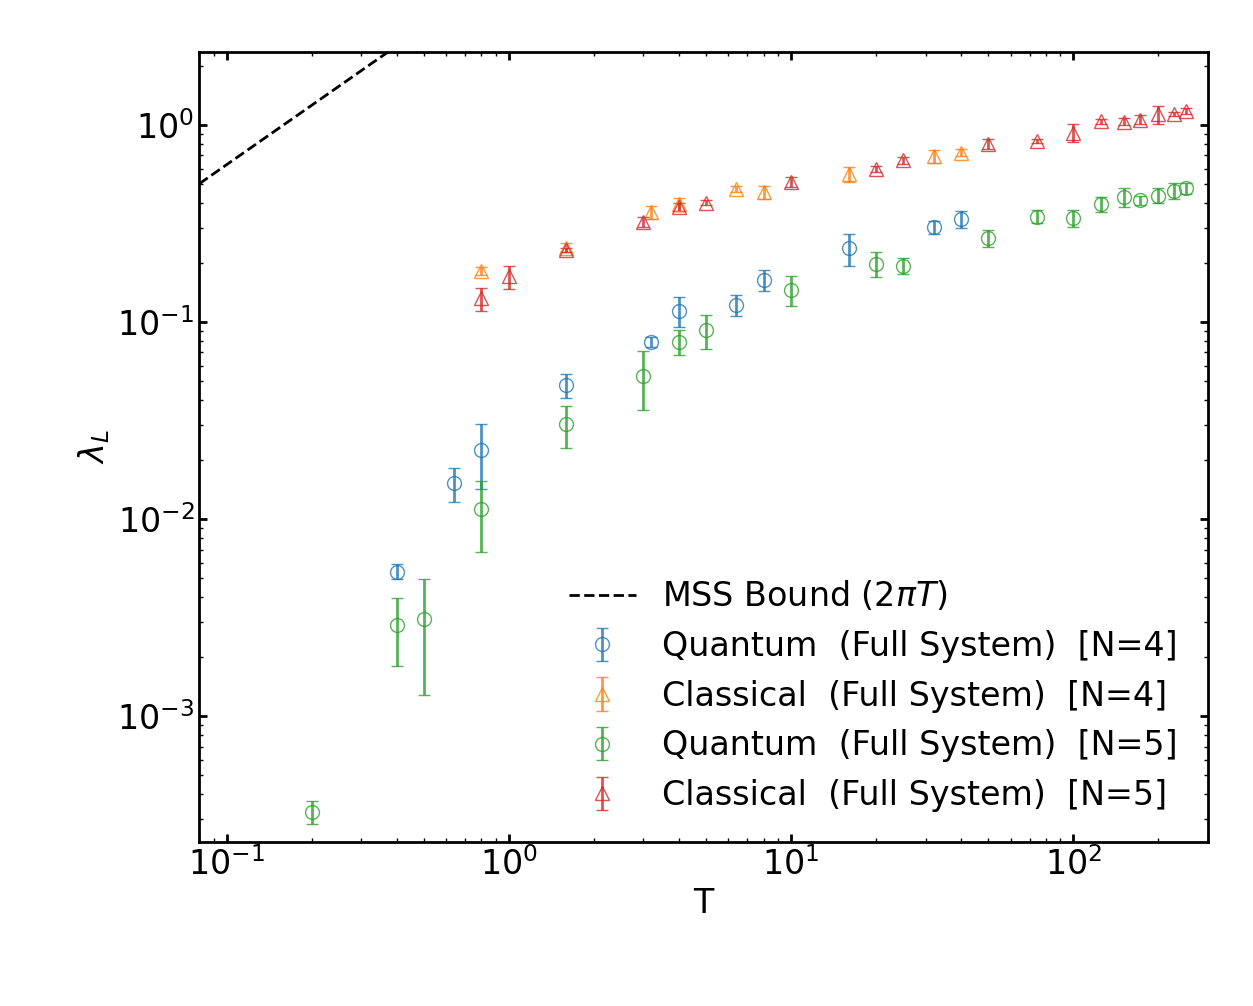
\includegraphics[width=\linewidth]{figures/LyapunovVsTNonPlanarN4N52.png}\\
      {\scriptsize \new{Full}: $N=4$ vs $N=5$.}
    \end{column}
    \begin{column}{0.33\textwidth}
      \centering
      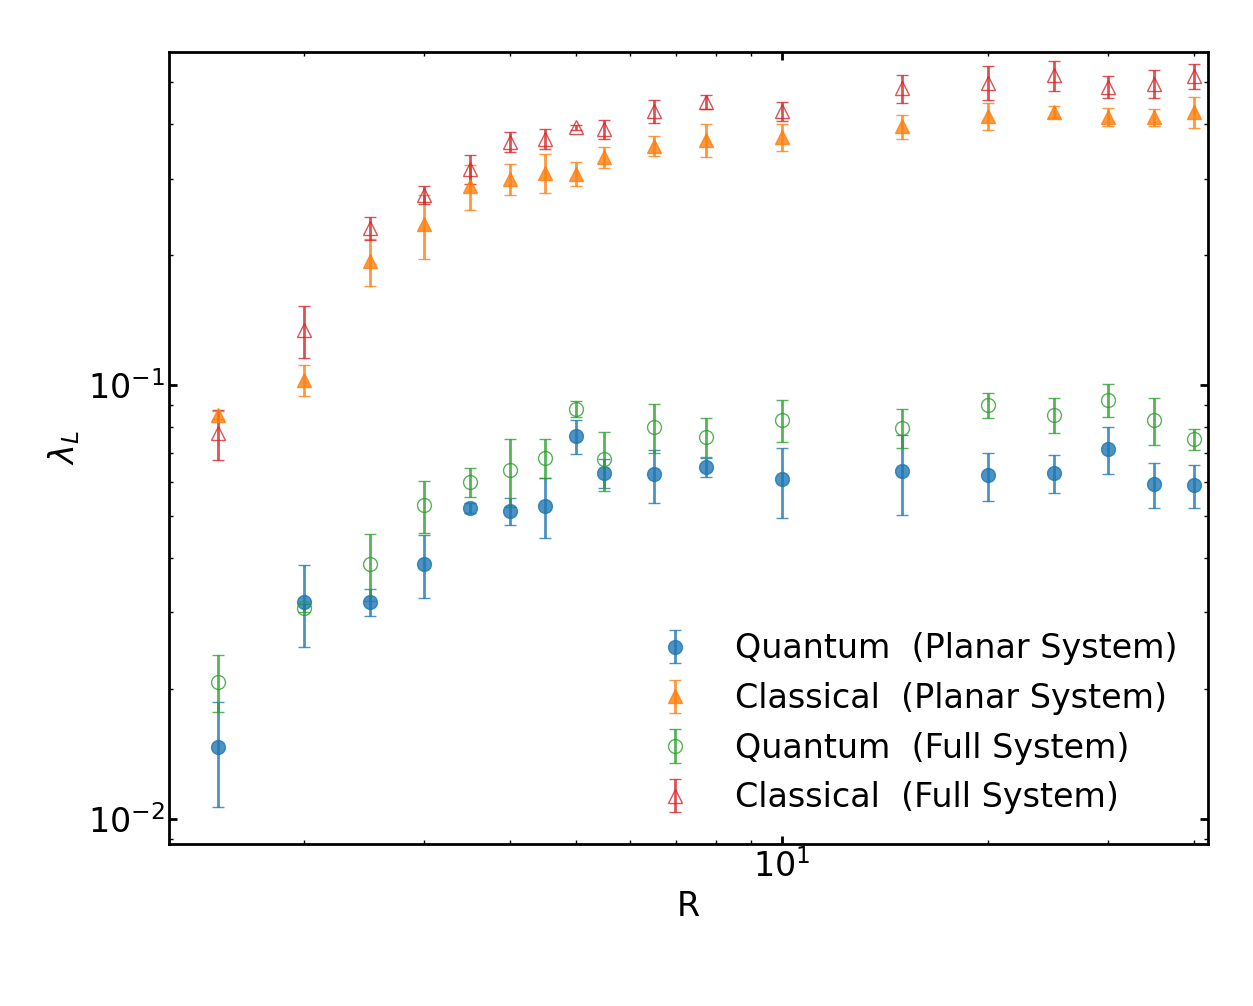
\includegraphics[width=\linewidth]{figures/LyapunovVsRPlanarNonPlanar.png}\\
      {\scriptsize $\lambda_L$ vs radius $R$ at $T=5$.}
    \end{column}
  \end{columns}
  \vspace{0.5em}
  \begin{itemize}\footnotesize
    \item \hl{$N$-scaling:} $\lambda_L$ scales alike at $N=4$ and $N=5$ for both interactions.
    \item \hl{Curvature:} $\lambda_L$ is steady for $R\gtrsim 3$, decreasing slowly for smaller $R$ -- the $l(l+1)/R^2$ term acts as an effective mass, driving the system more harmonic (less chaotic).
  \end{itemize}
\end{frame}

% ==============================================================
% Section 5: Entanglement
% ==============================================================
\section{Entanglement}

\begin{frame}{\new{Entanglement Entropy} via Reduced Covariance \newflag}
  \begin{block}{Why this is feasible}
    GSA is not unitary, but \hl{pure states stay pure} $\Rightarrow$ entanglement entropy is computable.
  \end{block}
  Sequence of bipartitions of the $2N^2$ modes by angular momentum:
  \begin{equation*}
    \mathcal{H}=\mathcal{H}_{\le L}\otimes\mathcal{H}_{>L},
    \qquad \mathcal{H}_{\le L}:\ \text{modes with } l\le L.
  \end{equation*}
  \begin{itemize}
    \item Reduced covariance $\Sigma_{\le L}$: restrict $\Sigma$ to the first $(L+1)^2$ modes.
    \item $S_{\le L}$ = von Neumann entropy from symplectic eigenvalues of $\Omega_{\le L}\Sigma_{\le L}(t)$.
    \item The \new{fuzzy structure} naturally plays the role of a lattice discretization, while keeping $SU(2)$ intact -- and the method applies directly to the \emph{interacting} theory.
  \end{itemize}
\end{frame}

\begin{frame}{Entanglement: Fast-Scrambling Behavior \newflag}
  \begin{figure}
    \captionsetup[subfigure]{skip=-10pt}   % ← default is ~10pt
    \centering
    \begin{subfigure}[b]{0.35\textwidth}
      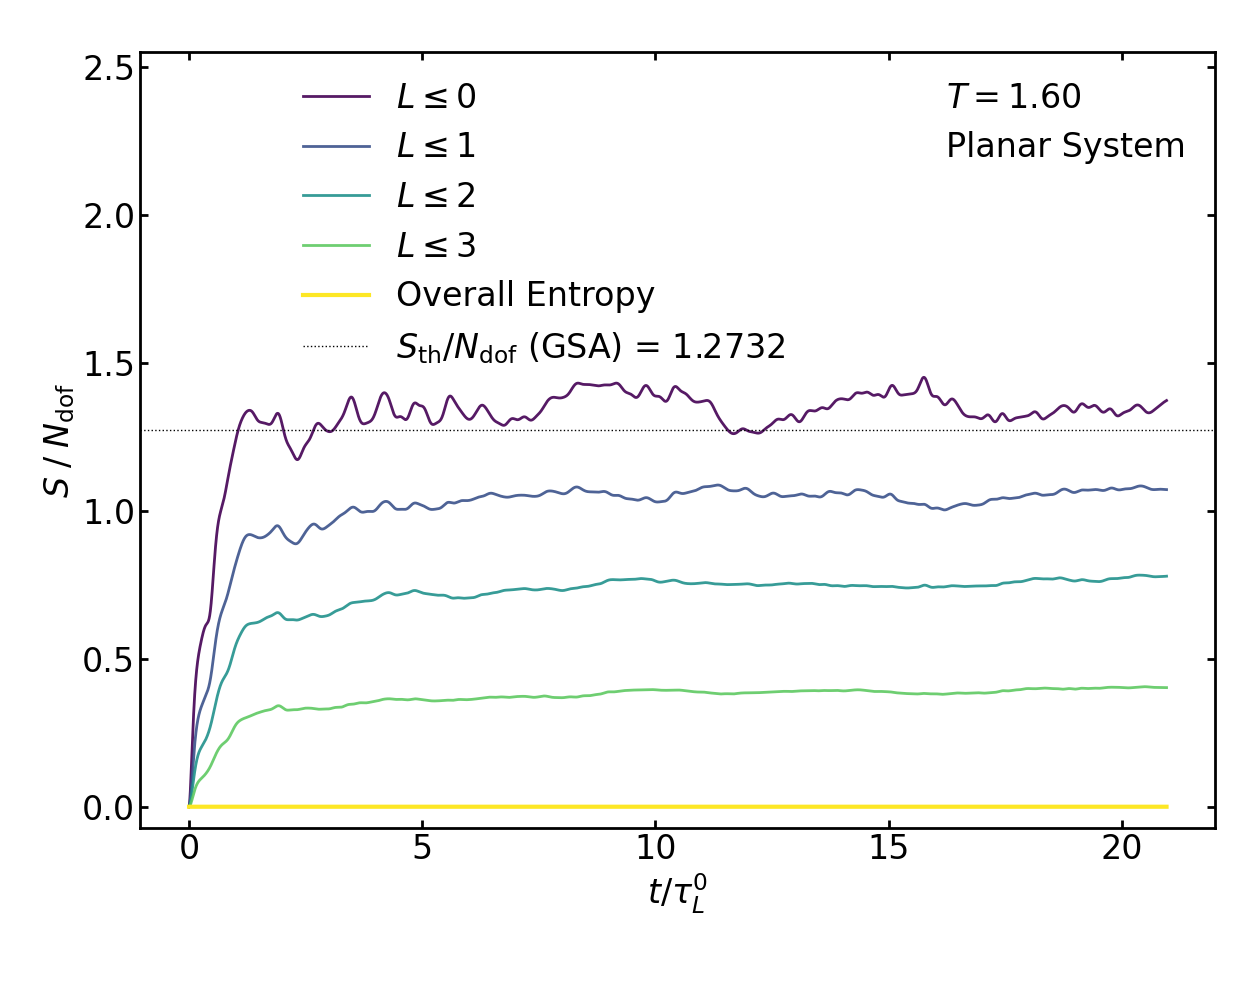
\includegraphics[width=\linewidth]{figures/EntropyVsTimeT16Planar.png}
      \caption*{\scriptsize Planar, $T=1.6$}
    \end{subfigure}\hfil
    \begin{subfigure}[b]{0.35\textwidth}
      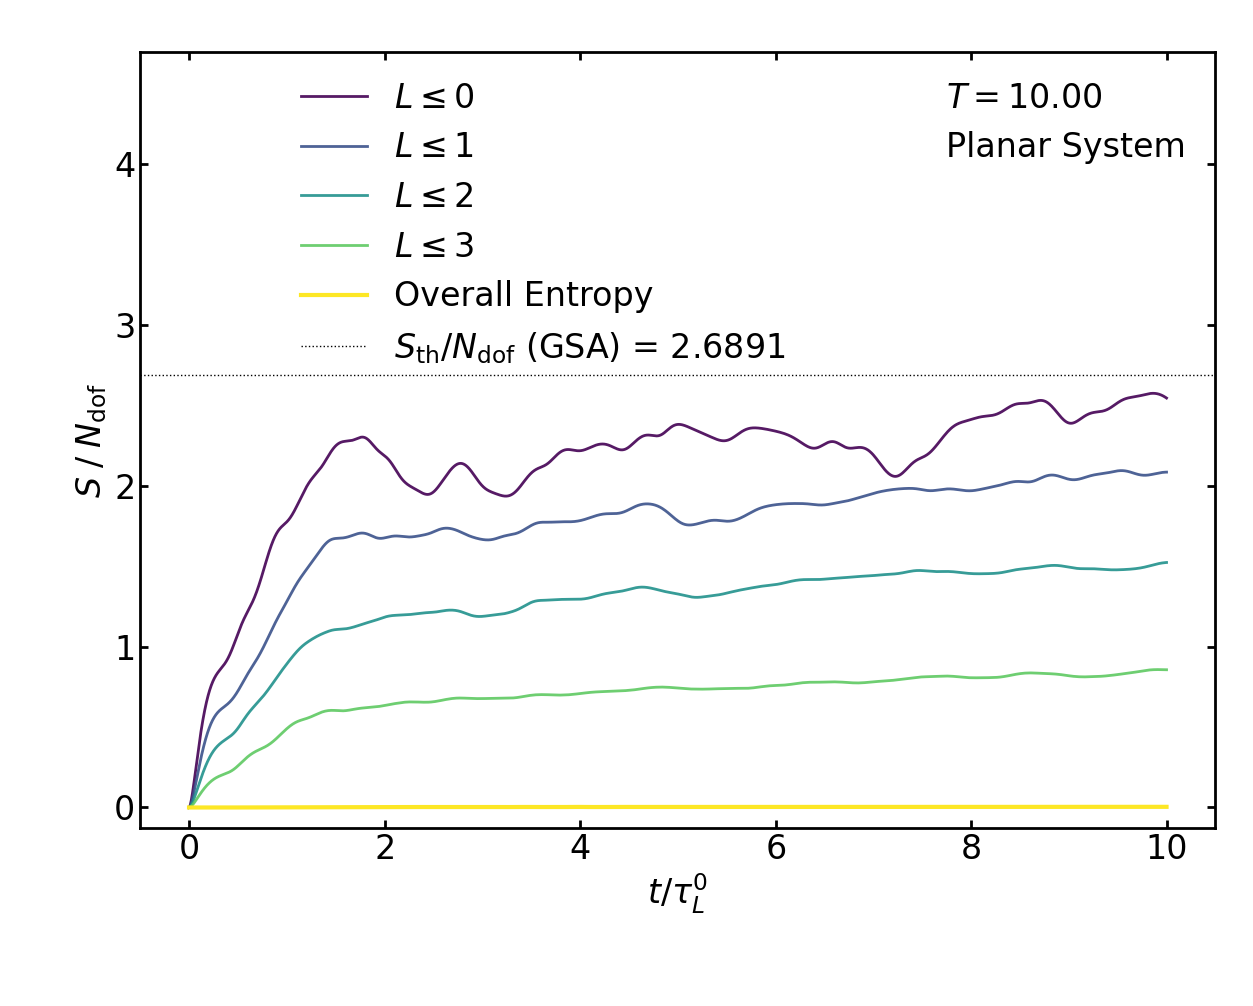
\includegraphics[width=\linewidth]{figures/EntropyVsTimeT10Planar.png}
      \caption*{\scriptsize Planar, $T=10$}
    \end{subfigure}\\[-0.8em]
    \begin{subfigure}[b]{0.35\textwidth}
      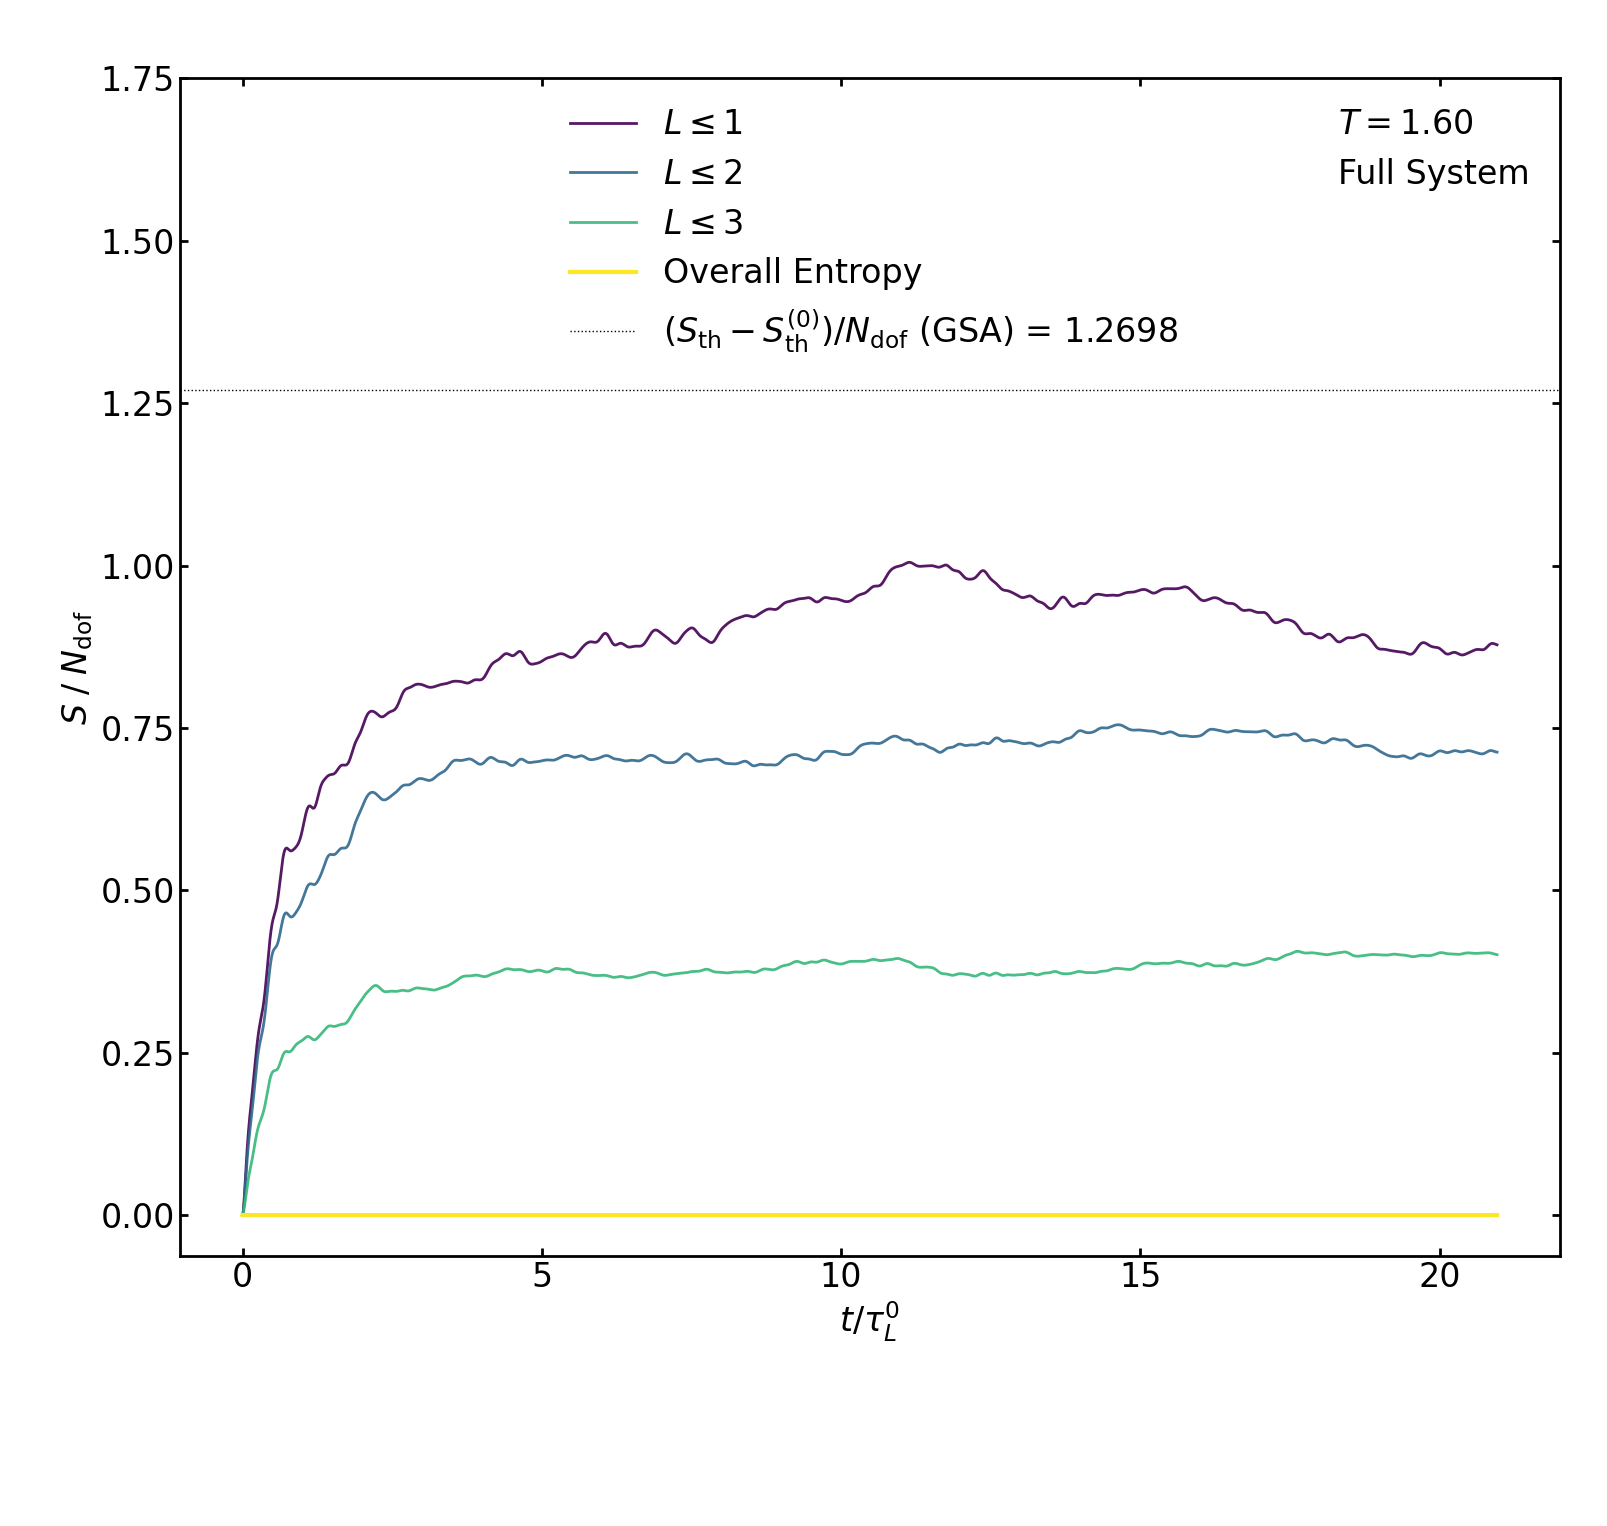
\includegraphics[width=\linewidth]{figures/EntropyVsTimeT16NonPlanar.png}
      \caption*{\scriptsize \new{Full}, $T=1.6$}
    \end{subfigure}\hfil
    \begin{subfigure}[b]{0.35\textwidth}
      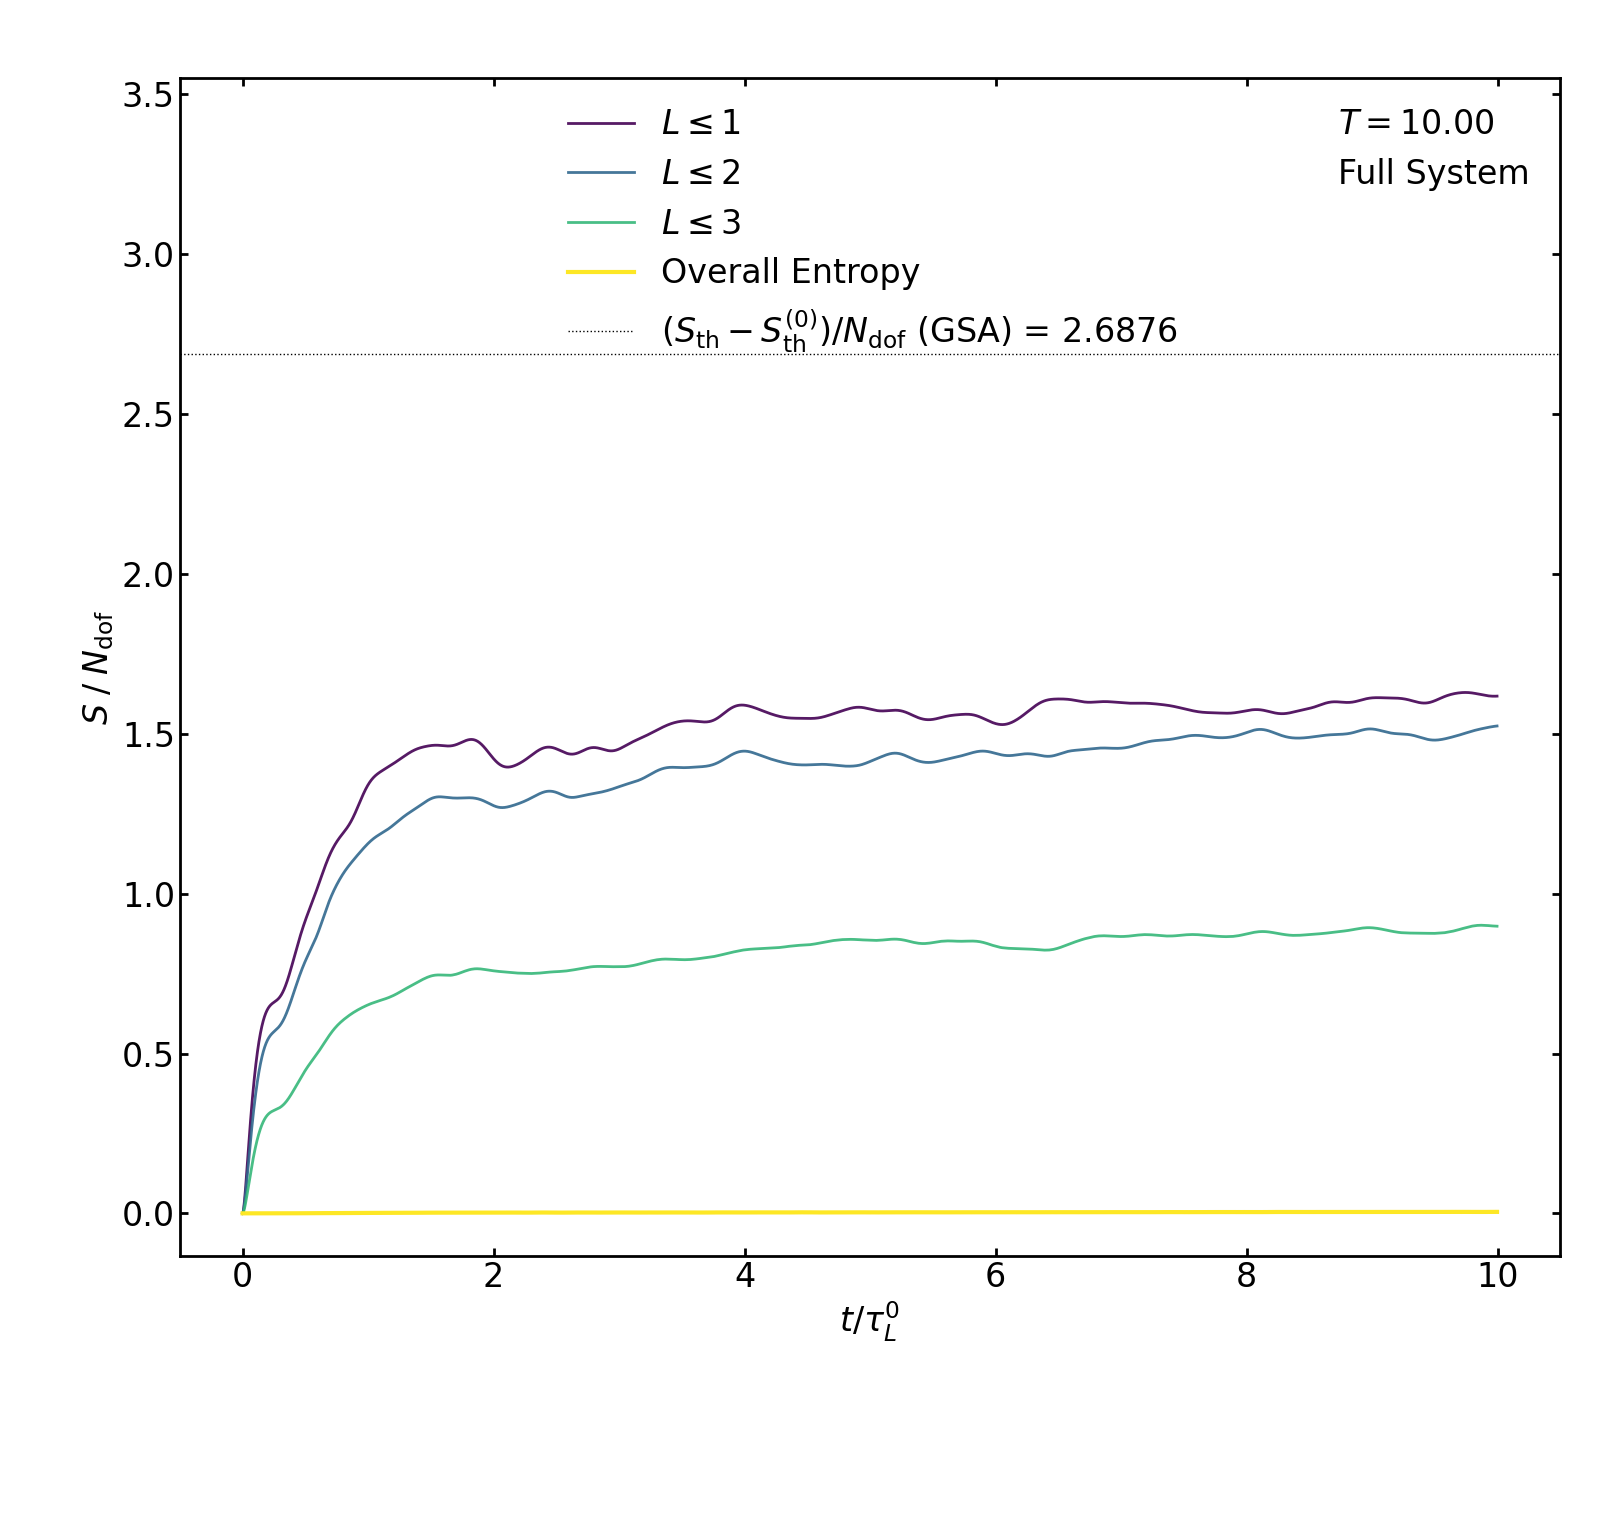
\includegraphics[width=\linewidth]{figures/EntropyVsTimeT10NonPlanar.png}
      \caption*{\scriptsize \new{Full}, $T=10$}
    \end{subfigure}
  \end{figure}
  \vspace{-0.3em}
  {\footnotesize $S_{\le L}/N_{\mathrm{dof}}$ vs time for $L=0,1,2,3$ (planar), $L=1,2,3$ (full). Sharp linear growth $\to$ saturation = hallmark of a fast scrambler. The pure-state line stays at zero (consistency check). Saturation $\to$ thermal entropy per dof.}
\end{frame}

\begin{frame}{Entanglement Saturation vs.\ Lyapunov: $\lambda_E$ vs $\lambda_L$ \newflag}
  \begin{columns}[T]
    \begin{column}{0.5\textwidth}
      \centering
      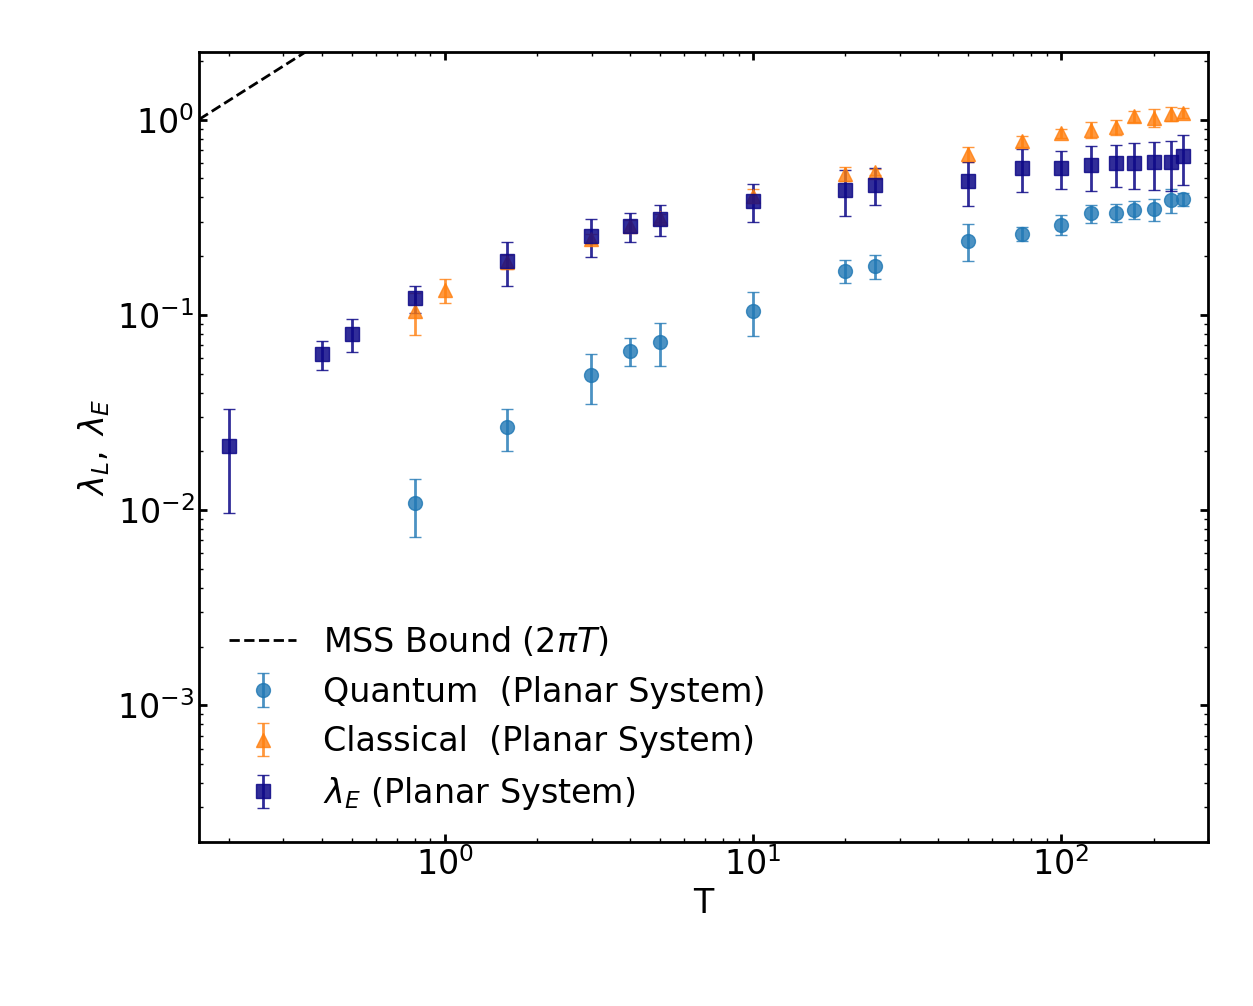
\includegraphics[width=\linewidth]{figures/LyapunovVsTPlanar2.png}\\
      {\scriptsize Planar System.}
    \end{column}
    \begin{column}{0.5\textwidth}
      \centering
      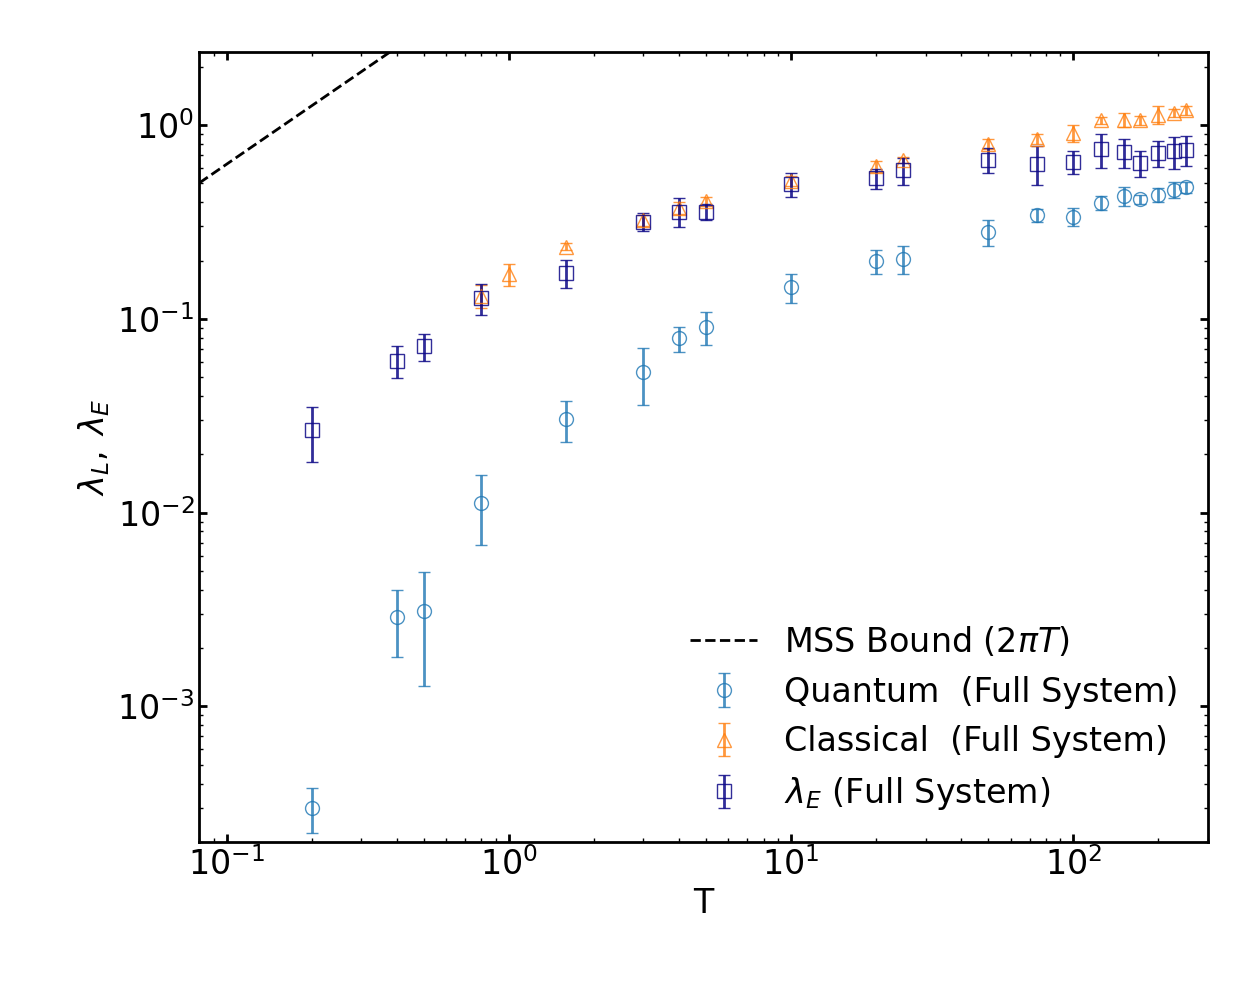
\includegraphics[width=\linewidth]{figures/LyapunovVsTNonPlanar2.png}\\
      {\scriptsize \new{Full} System.}
    \end{column}
  \end{columns}
  \vspace{0.3em}
  Fitting $S_{\le L}\sim\tilde S\tanh(t/\tau_E)$ defines $\lambda_E:=\tau_E^{-1}$:
  \begin{itemize}\footnotesize
    \item \hl{$\lambda_E>\lambda_L$ at all temperatures} -- entanglement saturates faster than trajectories diverge.
    \item $\lambda_E$ tracks the \emph{classical} $\lambda_L$; the gap widens as the system gets colder.
  \end{itemize}
\end{frame}

% ==============================================================
% Section 6: BMN Model (Ongoing)
% ==============================================================
\section{BMN Model}

\begin{frame}{The BMN Matrix Model: Why It Is the Natural Next Step \newflag}
  \begin{block}{What is the BMN model?}
    A \hl{mass deformation of BFSS} that maximally preserves supersymmetry. Its classical vacua are \new{fuzzy 2-spheres} -- exactly the geometry of our completed work.
  \end{block}
  \begin{itemize}
    \item Global symmetry \new{$SO(3)\times SO(6)$} (vs.\ $SO(2)$ in the bosonic model).
    \item Nine $N\times N$ Hermitian matrices $\hat X_I$, split as $a\in\{1,2,3\}$ ($SO(3)$), $\alpha\in\{4,\dots,9\}$ ($SO(6)$).
    \item Holographically related to black holes $\Rightarrow$ the prime target for testing the MSS bound.
  \end{itemize}
  \begin{center}
    \footnotesize\color{metugray}
    We have completed the full GSA derivation and the thermal-equilibrium analysis. Numerical work is underway.
  \end{center}
\end{frame}

\begin{frame}{The BMN Hamiltonian \newflag}
  \begin{equation*}
    \hat H=\frac{1}{2}\Tr\!\left(\hat P_I^2+\sum_{I=1}^{9}\Omega_I^2\hat X_I^2
      -\frac{\lambda}{2}\sum_{I\neq J}[\hat X_I,\hat X_J]^2
      +\tikzmarknode{M}{\frac{2i\mu\sqrt{\lambda}}{3}}\epsilon_{abc}\hat X_a\hat X_b\hat X_c\right)
  \end{equation*}
  \vspace{1.6cm}

  with $\Omega_I^2$ defined as
  \begin{equation*}
    \Omega_I^2=\begin{cases}\mu^2/9 & I\in\{1,2,3\}\\[2pt]\mu^2/36 & I\in\{4,\dots,9\}\end{cases}
  \end{equation*}

  \begin{tikzpicture}[overlay, remember picture]
    \draw[-stealth, shorten <=3pt, shorten >=2pt, thick, bend left=12]
      (M.south) to ++(-1.0,-0.8)
      node[below, font=\footnotesize, text width=4.7cm, align=center, fill=metulight, draw=metured, rounded corners, inner sep=5pt]{
        \new{Cubic term}: the new structural ingredient absent from the bosonic model.
      };
  \end{tikzpicture}

  \begin{itemize}\footnotesize
    \item The cubic term introduces the structure constant $\mathcal{F}^{l_1l_2l_3}_{m_1m_2m_3}=\Tr(Z_{l_1m_1}Z_{l_2m_2}Z_{l_3m_3})$.
    \item Symmetrized: $\widetilde{\mathcal{F}}^{l_1l_2l_3}_{m_1m_2m_3}=2\mathcal{F}^{l_1l_2l_3}_{m_1m_2m_3}-\mathcal{F}^{l_1l_3l_2}_{m_1m_3m_2}$.
  \end{itemize}
\end{frame}

\begin{frame}{BMN: Heisenberg \& One-Point EOM \newflag}
  Heisenberg EOM ($\partial_t\hat{\mathcal{O}}=-i[\hat{\mathcal{O}},\hat H]$) for the momentum:
  {\footnotesize
  \begin{equation*}
    \dot{\hat P}_K^{l_km_k}=-\Big[\Omega_K^2\hat X_K^{l_km_k}
      +i\tfrac{\mu\sqrt\lambda}{3}\epsilon_{Kbc}\widetilde{\mathcal{F}}\,\hat X_b\hat X_c
      -\tfrac{\lambda}{2}\mathcal{N}\,\hat X_J\hat X_K\hat X_J\Big].
  \end{equation*}}
  \begin{block}{GSA: mean-field + fluctuation decomposition}
    Write $\hat X=\bar X+\delta\hat X$ with $\bar X_I^{lm}=\braket{\hat X_I^{lm}}$, $\braket{\delta\hat X}=0$. Then the one-point $\braket{\hat P}$ EOM closes:
  \end{block}
  {\footnotesize
  \begin{align*}
    \dot{\bar P}_K^{l_km_k}=-\Big[\Omega_K^2\bar X_K^{l_km_k}
      &+i\tfrac{\mu\sqrt\lambda}{3}\epsilon_{Kbc}\widetilde{\mathcal{F}}\big(\bar X_b\bar X_c+\dbk{X_bX_c}\big)\\
      &-\tfrac{\lambda}{2}\mathcal{N}\big(\bar X_J\bar X_K\bar X_J+\dbk{X_JX_K}\bar X_J+\dots\big)\Big].
  \end{align*}}
  \vspace{-0.4em}
  {\footnotesize Each classical product is dressed by its 2-point (quantum) correction -- the GSA backreaction.}
\end{frame}

\begin{frame}{BMN: Two-Point EOM \newflag}
  Differentiating the connected covariances yields the kinematic relations
  {\small
  \begin{align*}
    \partial_t\dbk{X_I X_J} &= \dbk{P_I X_J}+\dbk{X_I P_J},\\
    \partial_t\dbk{X_I P_J} &= \dbk{P_I P_J}+\dbk{X_I\dot{\hat P}_J},\\
    \partial_t\dbk{P_I P_J} &= \dbk{\dot{\hat P}_I P_J}+\dbk{P_I\dot{\hat P}_J}.
  \end{align*}}
  The force-correlators $\dbk{X_I\dot{\hat P}_J}$, $\dbk{P_I\dot{\hat P}_J}$ are expanded term by term via Wick's theorem. The quartic piece contributes three pairing channels, e.g.
  {\footnotesize
  \begin{align*}
    \dbk{X_I\dot{\hat P}_J}_{\text{quart}}=\tfrac{\lambda}{2}\mathcal{N}\Big[
      &\dbk{X_IX_K}\bar X_J\bar X_K+\bar X_K\dbk{X_IX_J}\bar X_K+\dots\\
      &+\dbk{X_IX_K}\dbk{X_JX_K}+\dbk{X_IX_J}\dbk{X_KX_K}+\dots\Big].
  \end{align*}}
  \vspace{-0.5em}
  {\footnotesize $\Rightarrow$ The full closed truncated system for the BMN model has been derived (mass + cubic + quartic).}
\end{frame}

\begin{frame}{BMN Thermal Equilibrium: Non-Trivial Vacuum \newflag}
  \begin{alertblock}{Key difference from the bosonic model}
    The BMN classical vacuum is \hl{non-zero}: $\bar X_a^{\text{vac}}=\tfrac{\mu}{3\sqrt\lambda}L_a$, $\bar X_\alpha^{\text{vac}}=0$.
  \end{alertblock}
  Converting $L_a$ to the real polarization basis ($l=1$ sector only) gives the thermal one-point function
  \begin{equation*}
    \bar X_a^{lm}=\alpha\,\delta_{l,1}\,\Lambda_a^m,\qquad
    \alpha=\frac{\mu}{3\sqrt\lambda}\sqrt{\frac{S(S+1)(2S+1)}{3}},\quad S=\tfrac{N-1}{2}.
  \end{equation*}
  The unbroken symmetries reduce the covariance to a block-isotropic form with \new{two} species sectors:
  \begin{equation*}
    \dbk{X_I^{l_1m_1}X_J^{l_2m_2}}=\sigma_{xx}^{(I)}(l_1)\delta_{IJ}\delta^{l_1l_2}\delta^{m_1m_2},\quad
    \sigma^{(I)}=\begin{cases}\sigma^{(3)} & I\le 3\\ \sigma^{(6)} & I\ge 4\end{cases}
  \end{equation*}
\end{frame}

\begin{frame}{BMN: Energy Functional \& Gap Equations \newflag}
  The Gaussian energy functional (classical background drops out by stationarity):
  {\footnotesize
  \begin{align*}
    E[\vec\sigma]=\tfrac{1}{2}\sum_l(2l+1)\big[3\sigma_{pp}^{(3)}+6\sigma_{pp}^{(6)}\big]
      &+\tfrac{\mu^2}{6}C_3+\tfrac{\mu^2}{12}C_6\\
      &+\tfrac{\lambda}{2N}\big[6C_3^2+36C_3C_6+30C_6^2\big]+\dots
  \end{align*}}
  Entropy maximization $\Rightarrow$ \hl{gap equations} for the two frequency sectors:
  {\footnotesize
  \begin{align*}
    (\omega_l^{(3)})^2 &= \tfrac{\mu^2}{9}+\tfrac{2\lambda}{N}\big(2C_3^{\text{tot}}+6C_6\big)-2\lambda\big[2D^{(3),\text{tot}}(l)+6D^{(6)}(l)\big],\\
    (\omega_l^{(6)})^2 &= \tfrac{\mu^2}{36}+\tfrac{2\lambda}{N}\big(3C_3^{\text{tot}}+5C_6\big)-2\lambda\big[3D^{(3),\text{tot}}(l)+5D^{(6)}(l)\big].
  \end{align*}}
  closed by the \hl{coupled $2N$ self-consistency system}
  \begin{equation*}
    \sigma_{xx}^{(s)}(l)=\frac{1}{2\,\omega_l^{(s)}[\vec\sigma]}\coth\!\Big(\frac{\beta\,\omega_l^{(s)}[\vec\sigma]}{2}\Big),\quad s\in\{3,6\}.
  \end{equation*}
\end{frame}

% ==============================================================
% Section 7: Conclusion
% ==============================================================
\section{Conclusion}

\begin{frame}{Summary}
  \vspace{-0.9em}
  \begin{block}{Completed -- Bosonic model on $S_F^2\times\mathbb{R}$}
    \begin{itemize}
      \item Full GSA truncated EOM, thermal equation of state via entropy maximization.
      \item \new{Non-planar term included} -- not $1/N^2$-suppressed (only $SU(2)$ symmetry).
      \item $\lambda_L$ \hl{respects the MSS bound} at all $T$; vanishes at finite $T_c$.
      \item \new{Bekenstein bound satisfied}; \new{entanglement} shows fast scrambling with $\lambda_E>\lambda_L$.
      \item Manuscript prepared for submission.
    \end{itemize}
  \end{block}
  \vspace{-0.8em}
  \begin{block}{Ongoing -- BMN model}
    \begin{itemize}
      \item Full GSA EOMs and $SO(3)\times SO(6)$ thermal equilibrium \new{derived}.
      \item Gap equations \& coupled self-consistency system in hand.
    \end{itemize}
  \end{block}
\end{frame}

\begin{frame}{Timeline \& Outlook}
  \begin{center}
  \small
  \begin{tabular}{lll}
    \toprule
    \textbf{Task} & \textbf{Status} & \textbf{Target} \\
    \midrule
    Bosonic: GSA EOM + thermal equilibrium & \color{metured}Complete & --- \\
    Bosonic: Lyapunov + entanglement & \color{metured}Complete & --- \\
    Bosonic: Manuscript & \color{metured}Complete & Submitted \\
    \midrule
    BMN: GSA EOM derivation & \color{metured}Complete & --- \\
    BMN: Thermal equilibrium derivation & \color{metured}Complete & --- \\
    BMN: Self-consistency solver & \color{metugold}In progress & Q2 2026 \\
    BMN: Lyapunov computation (C++) & \color{metugold}In progress & Q2 2026 \\
    BMN: Entanglement entropy analysis & \color{metugray}Planned & Q2 2026 \\
    BMN: Manuscript & \color{metugray}Planned & Q3 2026 \\
    \midrule
    Parallel Project: TFD \& Bogoliubov tranformation& \color{metugray}Planned & Q4 2026 \\
    \midrule
    Thesis finalization & \color{metugray}Planned & May 2027 \\
    \bottomrule
  \end{tabular}
  \end{center}
  \vspace{0.5em}
\end{frame}

{
\setbeamertemplate{footline}{}
\setbeamertemplate{headline}{}
\begin{frame}
  \begin{center}
    \vspace{1.2cm}
    {\Large\color{metured}\textbf{Thank you!}}\\[0.6cm]
    {\large Questions \& Discussion}\\[1.2cm]
    
\includegraphics[height=1.6cm]{pic/METU_logo.png}\\[0.4cm]
    {\footnotesize Berk Özcan \quad$\cdot$\quad Supervisor: Prof.\ Dr.\ Seçkin Kürkçüoğlu}\\
    {\footnotesize Middle East Technical University -- Department of Physics}
  \end{center}
\end{frame}
}

\end{document}
